\chapter{Proof of Concept}
\label{sec:proofofconcept}

% PHP/XEDUB installation: https://ubuntuforums.org/showthread.php?t=525257
%						  https://www.youtube.com/watch?v=OlcsQ8TCU3A
%	> sudo add-apt-repository ppa:ondrej/php
%	> sudo apt-get update
%	> sudo apt-get apache2
% 	> sudo apt-get install php7.1-dev php-pear php7.1-mbstring php7.1-cgi	  			// old... > sudo apt-get install php5-dev php-pear
%	> sudo apt-get install libapache2-mod-php7.0
% 	> sudo pecl install xdebug
% 	> find / -name 'xdebug.so' 2> /dev/null
% 	/usr/lib/php5/20060613/xdebug.so
% 	> sudo gedit /etc/php/7.1/apache2/php.ini		
%		[xdebug]
%		zend_extension=/usr/lib/php/20160303/xdebug.so
%		xdebug.default_enable=1
%		xdebug.idekey=PHPSTORM
%		xdebug.remote_enable=1
%		xdebug.remote_port=9000
%		xdebug.remote_connect_back=1

% Enabling error msg. Set "`display_errors = On"' in:
%	> sudo gedit /etc/php/7.1/apache2/php.ini	

% Change document root:
% 	> sudo gedit /etc/apache2/sites-available/000-default.conf
%	> sudo gedit /etc/apache2/apache2.conf
% 	> sudo /etc/init.d/apache2 restart

% Installing grunt (as npm package):
%	> npm init
%	> npm install grunt --save-dev
%	create Gruntfile and update package.json according to: https://gruntjs.com/getting-started and http://www.wearecube.ch/from-less-to-css-with-grunt-js/
%	> npm install
%	> grunt
%					// > grunt watch &				// grunt watch will be stoped when the commandline closes

% installing composer/twig:
% 	download to project root: https://getcomposer.org
% 	> php composer-setup.php --filename=composer
%	create composer.json in project root. content:
% 		{
%			"require": {
%   			"twig/twig": "1.*",
%			    "twbs/bootstrap": "3.3.7"
%  			}
%		}
%	> php composer.phar install 		or			php composer.phar update
%	> sudo chown www-data:www-data bookinganalyzerimpl/compilation_cache/

% https://nikic.github.io/2011/12/12/How-big-are-PHP-arrays-really-Hint-BIG.html
% installing redis
%	> sudo pecl install redis
%	Adding "extension=redis.so" to php.ini
%	  	> sudo gedit /etc/php/7.1/apache2/php.ini	
%	  	> sudo gedit /etc/php/7.1/cli/php.ini	
% 	> sudo /etc/init.d/apache2 restart
%
%	> wget http://download.redis.io/releases/redis-3.2.8.tar.gz
%	> tar xzf redis-3.2.8.tar.gz
%	> cd redis-3.2.8
%	> make
% 	> ~/programs/redis-3.2.8/src/redis-server
% http://www.codeforge.com/article/214557


% Getting bookinganalyzerimpl to run:
% git clone git@github.com:soultemptation/bookinganalyzerimpl.git
% npm install
% grunt
% php composer.phar install

% Remove duplicates:
%			Find duplicates:
%			> egrep -o '^[^@]+' u611a_10_normalized_geocoded.csv > text.csv 	// Get everything before first @
%			> sort text.csv > text_sorted.csv									// Sort it
%			> uniq -d text_sorted.csv > text2_duplicates.csv					// Remove duplicates
% 	> tac u611a_10_normalized_geocoded.csv | sort -k1,1 -r -u -t@ > text5.csv
%	> tac text5.csv > text6.csv
%	Move last line of text6.csv to the beginning

\section{Datenvorbereitung}
\label{sec:proofofconcept:datenvorbereitung}

% Feature selection
% https://en.wikipedia.org/wiki/Feature_selection
% http://dollar.biz.uiowa.edu/~street/research/dmoc.pdf
% http://www.jmlr.org/papers/volume3/guyon03a/guyon03a.pdf

Die Daten müssen für die Verwendung im Proof of Concept vorbereitet werden. Dazu wurden zwei Programme geschrieben um die Daten anzureichern. Die Datentransormationen wurden anschliessend gemäss \cref{sec:recherche:datenvorbereitung} mit dem Programm RapidMiner durchgeführt.

\subsection{Datenerweiterung}
\label{sec:proofofconcept:datenvorbereitung:datenerweiterung}
Die Programme für die Datenanreicherungen sind jeweils eine Kommandozeilen-Software welche hier vorgestellt werden.

\subsubsection{Land, Region, Ortschaft}
\label{sec:proofofconcept:datenvorbereitung:datenerweiterung:landregionortschaft}
Es wurde ein Programm für die Anreicherung vom Land, der Region sowie der Ortschaft der Objekte erstellt. Es erwartet eine \gls{csv} Datei mit einem @-Zeichen als Feldseparator, sowie das Feld "`NREF"' welches in jeder Zeile vorkommen muss und die ID des Objektes beinhaltet. Der Quellcode ist einsehbar in Github unter \url{https://github.com/soultemptation/bookinganalyzerdestinations}.

Die Software verarbeitet Zeile für Zeile der Datei und fügt am Ende drei Felder mit den Namen "`country"', "`region"' und "`place"' an. Um die Daten zu erhalten wird der Such-Service von Interhome angesprochen, welcher die drei Informationen zurückliefert. Als Parameter des Services wird die `NREF"' des Objektes übergeben. 

Es kann sein dass das Objekt bei Interhome nicht mehr vorhanden ist und der Service nichts zurück liefert. Deshalb gibt es nach der Ausführung des Programmes Buchungen welche keine Informationen für das Land, die Region und die Ortschaft besitzen.

Im Programm wird ein Cache verwendet, welcher für jede "`NREF"' das Land, die Region und die Ortschaft zwischenspeichert. Wenn eine "`NREF"' zum zweiten mal angefragt werden soll, können die Daten aus dem Cache bezogen werden und es muss kein weiterer Service Aufruf durchgeführt werden. Für die 133'001 Buchungen mussten dank des Caches nur 78'342 Anfragen an den Service gestellt werden.

\subsubsection{Geolocation}
\label{sec:proofofconcept:datenvorbereitung:datenerweiterung:geolocation}
Das Programm für die Anreicherung der Geolocation erwartet wie die im \cref{sec:proofofconcept:datenvorbereitung:datenerweiterung:landregionortschaft} vorgestellte Software eine \gls{csv} Datei, in welchem die Felder mit einem @-Zeichen getrennt sind, sowie die Attribute "`CUSTRAS"' (Strasse), "`CUCNTRY"' (Land), "`CUZIP"' (Postleitzahl) und "`CUORT"' (Ort). Unter \url{https://github.com/soultemptation/BookingAnalyzerGeocoding} ist der Quellcode abgelegt. 

Um die Adresse in Geo-Koordinaten umzuwandeln wurde die "`Locations API"' von Bing Maps (Microsoft) verwendet (siehe \url{https://msdn.microsoft.com/en-us/library/ff701715.aspx}). Da der Service nicht kostenlos ist und 133'001 Geocoding-Anfragen gesendet werden mussten, wurde eine Lizenz benötigt welche an einen "`API Key"' gebunden ist. Es konnte eine Studenten-Lizenz erworben werden, welcher 10'000 Anfragen pro Tag erlaubt.

Das Programm geht jede Zeile der Datenquelle durch und sendet eine Anfrage an die "`Locations API"'. Übergeben wird die Adresse des Kunden sowie ein "`API Key"' für die Authentifizierung. Die Anfrage ist folgendermassen aufgebaut:

\blockquote[]{http://dev.virtualearth.net/REST/v1/Locations?countryRegion=\textbf{\{Zweistelliger Ländercode\}}\&locality=\textbf{\{Stadt\}}\&postalCode=\textbf{\{Postleitzahl\}}\&addressLine=\textbf{\{Strasse und Hausnummer\}}\&includeNeighborhood=0\&maxResults=1\&key=\textbf{\{API Key\}}}

Um zum Beispiel die Geolocation der ZHAW Zürich anzufragen, kann folgender Request angesetzt werden:

\blockquote[]{http://dev.virtualearth.net/REST/v1/Locations?countryRegion=\textbf{CH}\&locality=\textbf{Zurich} \&postalCode=\textbf{8021}\&addressLine=\textbf{Lagerstrasse 41}\&includeNeighborhood=0\&max Results=1\&key=\{API Key\}}

Bing Maps liefert dafür die Koordinaten "`47.37766, 8.53259"' zurück. In der \cref{fig:proofofconcept:datenvorbereitung:datenerweiterung:geolocation:1} ist die Adresse auf einer Karte eingezeichnet.

\begin{figure}[H]
	\RawFloats
	\centering
	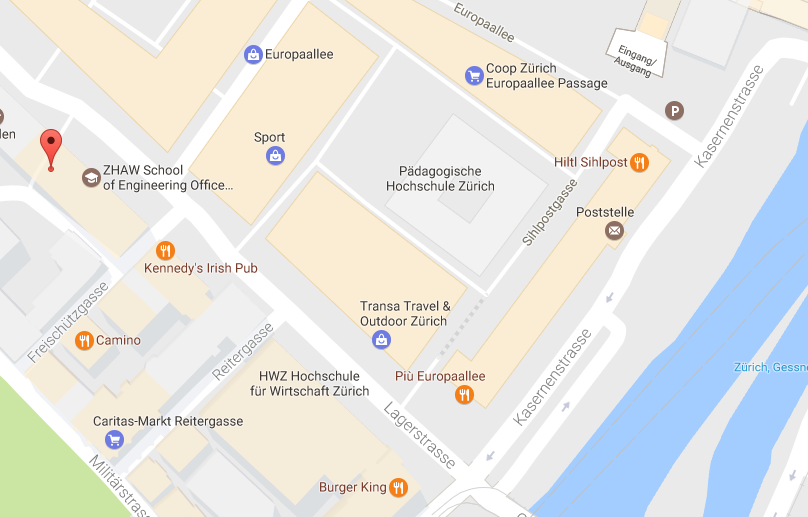
\includegraphics[width=1\textwidth]{images/bing-maps-result}
	\caption{Resultat des Geocodings von Bing Maps.}
	\label{fig:proofofconcept:datenvorbereitung:datenerweiterung:geolocation:1}
\end{figure}

\subsection{Datenvorbereitung mit RapidMiner}
Im \cref{sec:recherche:datenvorbereitung} wurde beschrieben, wie die Daten vorbereitet werden sollen. Dieser Abschnitt zeigt auf wie das Program RapidMiner verwendet wurde um diese Vorgaben zu erfüllen. \cref{fig:recherche:rapidminer:1} zeigt den definierte Prozess auf.

%Zuerst werden die Daten aus dem \gls{csv} File geladen. Anschliessend die Attribute gemäss \cref{fig:recherche:attributeinschraenkung:2} eingeschränkt sowie die Diskretisierung entsprechend \cref{fig:recherche:datenvorbereitung:1} und \ref{fig:recherche:datenvorbereitung:2} durchgeführt.

\begin{figure}[htb]
	\begin{subfigure}[t]{1\textwidth}
		\centering
		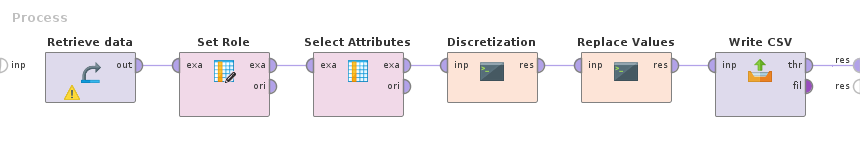
\includegraphics[width=1\textwidth]{images/rapidminer-process}
		\caption{Hauptprocess}
		\label{fig:recherche:rapidminer:1:1}
	\end{subfigure} \\
	\begin{subfigure}[t]{0.5\textwidth}
		\centering
		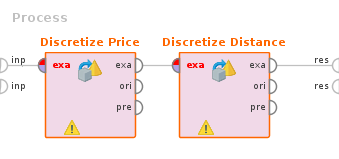
\includegraphics[width=1\textwidth]{images/rapidminer-process-discretization}
		\caption{Subprocess für die Diskretisierung}
		\label{fig:recherche:rapidminer:1:2}
	\end{subfigure}
	\begin{subfigure}[t]{0.8\textwidth}
		\centering
		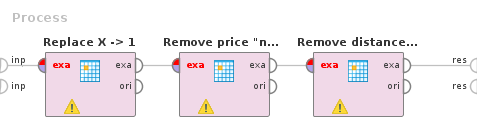
\includegraphics[width=1\textwidth]{images/rapidminer-process-replace-values}
		\caption{Subprocess für die Ersetzung von Attributwerten}
		\label{fig:recherche:rapidminer:1:3}
	\end{subfigure}
	\caption{RapidMiner Prozess für die Vorbereitung der Daten}
	\label{fig:recherche:rapidminer:1}
\end{figure}

 In \ref{fig:recherche:rapidminer:1:1} wird der Hauptprozess gezeigt wie er im RapidMiner definiert wurde. Nachfolgend werden die einzelnen Schritte 
 \begin{itemize}
 	\item Retrieve data: Lädt die Buchungen aus der Datenquelle damit diese bearbeitet werden können. 
 	\item Filter Exapmles: Entfernt alle Buchungen mit dem Status "`XX"' (siehe \cref{sec:recherche:datenvorbereitung:filtrieren} \nameref{sec:recherche:datenvorbereitung:filtrieren}).
 	\item Select Attribute: Entfernt alle Attribute welche nicht in der \cref{fig:recherche:attributeinschraenkung:2} ausfgewählführt werden, sind die Informationen nachher voll anonymisiert und können auch veröffentlicht werden. Der letzte Schritt schreibt das Resultat in ein \gls{csv} File damit es nachher weiterverwendet werden kann.
 	\item Generate ID: Generiert eine ID für die eindeutige Identifikation der Buchungen.
 	\item Normalize: Normiert nummerische Werte auf einen Interval $0 \leq x \leq 1$ (siehe \cref{sec:recherche:datenvorbereitung:normierung} \nameref{sec:recherche:datenvorbereitung:normierung}).
 	\item Weeklyprice: Berechnet den Wochenpreis einer Buchung (siehe \cref{sec:recherche:datenvorbereitung:normierung} \nameref{sec:recherche:datenvorbereitung:normierung}).
 	\item Discretization: Ist ein Unterprozess welcher in \cref{fig:recherche:rapidminer:1:2} dargestellt ist.
	 	\begin{itemize}
	 		\item Discretize Price: Diskretiert die Preise gemäss \cref{fig:recherche:datenvorbereitung:2}. Die Preisspannen die nicht im Resultat verwendet werden sollen werden später im Schritt "`Replace Values"' entfernt.
	 		\item Discretize Distance: Diskretiert die Distanzen gemäss \cref{fig:recherche:datenvorbereitung:1}. Distanzspannen die nicht im Resultat verwendet werden sollen werden später im Schritt "`Replace Values"' entfernt.
	 	\end{itemize}
 	\item Replace Values: Ist ein Unterprozess welcher in \cref{fig:recherche:rapidminer:1:3} dargestellt ist.
 		\begin{itemize}
			\item Replace X -> 1 und Replace empty -> 0: Wandelt boolsche Werte in 1 und 0 um (siehe \cref{sec:recherche:datenvorbereitung:boolschewerte} \nameref{sec:recherche:datenvorbereitung:boolschewerte}). 
			\item Remove price "normal": Bei der diskretierung des Preises sollen nur günstige und luxus Buchungen beachtet werden (siehe \cref{sec:recherche:datenvorbereitung:diskretierung} \nameref{sec:recherche:datenvorbereitung:diskretierung}). Mittlere Werte werden deshalb in diesem Schritt entfernt.
			\item Remove distance 499<: Gleich wie für den Preis werden Distanzen mit einem grösseren Wert als 499 nicht verwendet und deshalb in diesem Schritt entfernt.
 		\end{itemize}
 	\item Remove Price: Entfernt den gesamt Preis der Buchung. Dieser muss beim Schritt "`Select Attribute"' hinzugefügt werden damit der Wochenpreis berechnet werden kann. Im Resultat wird das Attribut jedoch nicht mehr benötig.
 	\item Write CSV: Speichert das Resultat im \gls{csv} Format auf die Festplatte ab.
 \end{itemize}

\section{Architektur}
\label{sec:proofofconcept:architektur}
Zuerst werden in diesem Abschnitt die wesentlichen Punkte aufgeführt, welche im \cref{sec:konzept} definiert wurden und Einfluss auf die Architektur genommen haben, und wie sie den Aufbau mitbestimmt haben. 
Anschliessend wird anhand eines \gls{uml}-Paketdiagrammes die Architektur visualisiert.

\subsection{Anforderungen aus dem Konzept}
\label{sec:proofofconcept:architektur:anforderungen}
Nachfolgend sind die Punkte aus dem \cref{sec:konzept} aufgeführt welche den grundsätzlichen Aufbau der Umsetzung bestimmen.

\begin{itemize}
	\item Ansichten: Es gibt vier Ansichten welche der Benutzer aufrufen kann. Stammdaten einsehen, Attributanalyse durchführen, Attributanalyse mit Gruppierung durchführen und Einstellungen anpassen.
	\item Datentypen der Stammdaten: Die Datenbasis besteht aus Daten welche verschiedene Datentypen annehmen können.
	\item Algorithmen: Es gibt drei Algorithmen welche auf die Datenbasis angewendet werden können: Apriori, KPrototype und DBScan.
	\item Filtrierung: Vor jeder Analyse kann die Datenbasis durch filter eingeschränkt werden.
	\item Konfiguration: Die Algorithmen sollen vom Endbenutzer konfigurierbar sein.
\end{itemize}

\subsubsection{Ansichten}
\label{sec:proofofconcept:architektur:anforderungen:ansichten}
Für die Darstellung der vier Ansichten (Stammdaten einsehen, Attributanalyse durchführen, Attributanalyse mit Gruppierung durchführen und Einstellungen anpassen) wird eine Lösung angestrebt, welche die Ansicht von der Applikationslogik trennt. Dazu wird eine Templating Bibliothek für die Darstellung verwendet mit welcher die Ansichten generiert werden können. 

Es wurden drei Bibliotheken evaluiert welche für die Erstellung der Ansichten verwendet werden können. Diese werden in den Kategorien Syntax, Funktionalität und Dokumention bewertet. Den ersten Punkt objektiv zu bewerten ist relativ schwierig. Es wurde versucht im Vergleich zu den anderen Kandidaten ein Urteil zu fällen wie verständlich die Templates zu lesen sind. Bei der Funktionalität wir der Funktionsumfang der einzelnen Bibliotheken miteinander verglichen. Die Dokumentation schlussendlich bewertet wie verständlich die Dokumentation zu lesen ist und wie tief sie reicht. Die Bewertungsskala reicht von 1 bis 9. 1-3 ist schlecht und beduetet dass der Punkt eine echtes Hindernis darstellt. 4-6 ist im Mittelfeld. Mit solch einer Benotung kann die Bibliothek eingesetzt werden, auch wenn Verbesserungen in dem Bereich erwünscht sind. 7-9 steht dafür, dass die Library in dem Bereich sehr gut ist im Vergleich mit den Konkurrenten
\begin{table}[H] 
	\caption{Vergleich verschiedener Templating Bibliotheken}
	\centering
	\rowcolors{1}{tablebodycolor}{tablerowcolor}
	\label{fig:proofofconcept:architektur:anforderungen:ansichten:1}
	\begin{tabular}{ | c | c | c | c | c | } 
		\hline 		
		\rowcolor{tableheadcolor}
		\bfseries Name & \bfseries Syntax & \bfseries Funktionalität & \bfseries Dokumentation & \bfseries Durchschnitt \\ \hline 
		
		Blade & \cellcolor{red!25}3 & \cellcolor{green!25}9 & \cellcolor{green!25}7 & \cellcolor{yellow!25}6.3\\ \hline 
		Mustache & \cellcolor{yellow!25}7 & \cellcolor{red!25}1 & \cellcolor{green!25}9 & \cellcolor{yellow!25}5.7\\ \hline 
		Twig & \cellcolor{green!25}6 & \cellcolor{green!25}9 & \cellcolor{green!25}9 & \cellcolor{green!25}8 \\ \hline 
	\end{tabular}
\end{table}

Blade (\url{https://laravel.com/docs/5.4/blade}) bietet eine herausragende Funktionalität an. Es werden die üblichen Befehle für die Ausgabe von Variablen, die Iteration über Listen und die IF/ELSE abfragen unterstützt. Zusätzlich können Grundgerüste erstellt werden welche später von einem anderen Template mit Daten befüllt werden. Dadurch kann in einer Datei der Grundaufbau der Seite definiert werden welche Bereiche definiert, welche später mit Inhalt befüllt werden. Dies fördert den modularen Aufbau massiv. Die Syntax jedoch ist sehr unleserlich. Die Verwendung von `Sections"' (siehe \url{https://laravel.com/docs/5.4/blade}) ist ein zentraler Bestandteil der Bibliothek aber die Verwendung ist schwer leserlich. Die Dokumentation schlussendlich ist sehr übersichtlich, jedoch sind einige detaillierteren Funktionalitäten ausgelassen worden.

Mustache (\url{https://mustache.github.io}) ist eine Library welche in über 30 Programmiersprachen portiert wurde. Deshalb ist die Dokumentation dazu auch sehr detailliert und gut verständlich. An Funktionalität bietet Mustache jedoch nur die Ausgabe von Variablen, eine Funktion zum Iterieren und eine Überprüfung ob ein Wert "`null"' ist. Da sind die beiden Kontrahenten um einiges stärker. Die Syntax ist leserlich und einfach verständlich, unter anderem auch weil die Funktionalität sehr eingeschränkt ist.

Twig (\url{https://twig.sensiolabs.org}) wurde inspieriert von Jinja, einer Templating Engine für die Programmiersprache Python. Die Syntax ist gut verständlich und sehr ähnlich zu jener von Mustache. Da jedoch die Funktionalität um einiges umfangreicher ausfällt wird auch die Verständlichkeit etwas beeinträchtigt. Wie gesagt die ist Funktionalität besser als bei Mustache, genauer gesagt ist sie hervorragend. Vergleichbar mit jener von Blade weshalb sie beide eine 9 erhalten. Im vergleich mit den anderen Kandidaten ist die Dokumentation am umfangreichsten und generell sehr verständlich.

Fazit: Eingesetzt wird Twig, weil es eine herausragende Dokumentation und Funktionsumfang bietet, welche über einige Schwächen beim Syntax hinwegzutäuschen vermag. Mehr zur Umsetzung der Ansichten mit Twig kann im \cref{sec:proofofconcept:externebibliotheken:twig} nachgelesen werden.

\subsubsection{Datentypen der Stammdaten}
\label{sec:proofofconcept:architektur:anforderungen:datentypen}
Bislang wurde von numerischen und kategorischen Attributen gesprochen. Dies ist ausreichend für die Definition der Algorithmen. Bei der Programmierung werden jedoch weitere Datentypen benötigt.

\begin{table}[H] 
	\caption{Datenbestand vor der Anwendung der Filterkriterien}
	\centering
	\rowcolors{1}{tablebodycolor}{tablerowcolor}
	\label{fig:proofofconcept:architektur:anforderungen:datetypen:1}
	\begin{tabular}{ | c | c | c | c | } 
		\hline 		
		\rowcolor{tableheadcolor}
		\bfseries Datentyp & Beschreibung & Wertebereich/Genauigkeit  \\ \hline 
		
		Integer & Numerische Werte & $-2^{63}-1$ bis $+2^{63}-1$ \\ \hline 
		String & Texte & $2^{31}-1$ bytes (2GB) \\ \hline 
		Float & Fliesskomma Zahlen & $1.11^{-16}$ \\ \hline 
		Boolean & Wahr oder falsch & true/false \\ \hline  
		Distance & Objekt vom Typ Distance & Close/[leer] \\ \hline 
		Price & Objekt vom Typ Price & Luxury/Budget \\ \hline 		
	\end{tabular}
\end{table}

Die Algorithmen behandelt Integer und Float als numerische-, und Boolean, Distance und Price als kategorische Attribute. Das Programm benötigt jedoch eine Unterscheidung dieser Typen da sie in verschiedene Datentypen abgelegt werden müssen. Zusätzlich werden noch Texte benötigt, welche zwar nicht analysiert, jedoch für die Filtrierung notwendig sind.

In der Umsetzung sind die Datentypen im Package "`Models"' abgelegt. Siehe \cref{sec:proofofconcept:packagestruktur} \nameref{sec:proofofconcept:packagestruktur} für eine Übersicht oder \cref{sec:proofofconcept:klassenstruktur:models} \nameref{sec:proofofconcept:klassenstruktur:models} für eine detaillierte Aufstellung.

\subsubsection{Algorithmen}
\label{sec:proofofconcept:architektur:anforderungen:algorithmen}
Den grössten Einfluss auf die Architektur haben die Algorithmen. Eine Webanfrage hat normalerweise eine obere Laufzeitgrenze von 30 Sekunden. Bis dann muss der Server eine Antwort liefern, sonst wird dem Benutzer eine Fehlermeldung angezeigt und der Prozess auf dem Server gestoppt. Da die Analyse, je nach Datenmenge, einige Minuten bis Stunden dauern kann musste dafür eine Lösung gefunden werden. 

Umgangen wurde diese Problematik durch den Einsatz von Hintergrundprozessen. Wenn der User auf einer Ansicht die Filter ausfüllt und den Analyseprozess startet wird ein Prozess auf dem Server gestartet und dem Benutzer eine Seite angezeigt mit der Info, dass die Analyse gestartet wurde. Der Prozess läuft dann im Hintergrund weiter und sendet dem Benutzer regelmässige Aktualisierungen über den Vorgang der Analyse. Mehr dazu im \cref{sec:proofofconcept:kommunikationsablauf} \nameref{sec:proofofconcept:kommunikationsablauf}.

\subsubsection{Filtrierung}
\label{sec:proofofconcept:architektur:anforderungen:filtrierung}
Um die Analyse durch Algorithmen auf einer Untermenge der Daten durchzuführen (siehe FA3 in im \cref{sec:anforderungsanalyse:funktionaleanforderung} \nameref{sec:anforderungsanalyse:funktionaleanforderung}) soll der User die Möglichkeit erhalten durch Einschränkung der Daten diese zu filtrieren. 

Deshalb wird in jeder Ansicht (ausser beim anpassen der Einstellungen) ein Formular angezeigt mit welcher die Daten eingeschränkt werden können. In der Umsetzung wurde ein Model erstellt welches die Filter für die verschiedenen Attribute abbildet (siehe \cref{sec:proofofconcept:klassenstruktur:models} \nameref{sec:proofofconcept:klassenstruktur:models}) und ein Twig Template um das Formular darzustellen (siehe \cref{sec:proofofconcept:externebibliotheken:twig} \nameref{sec:proofofconcept:externebibliotheken:twig}). Schlussendlich muss beim Zugriff der Daten die Filters beachtet werden. Es dürfen nur diejenigen Buchungen geliefert werden welche allen Kriterien zutreffen. Die Datenmengen auf die die Filter angewendet wurden werden gecached um den Zugriff zu beschleunigen (siehe \cref{sec:proofofconcept:performance:caching} \nameref{sec:proofofconcept:performance:caching}).

\subsubsection{Konfiguration}
Ein Benutzer des Programmes soll, das Programm konfigurieren können (siehe FA7 im \cref{sec:anforderungsanalyse:funktionaleanforderung} \nameref{sec:anforderungsanalyse:funktionaleanforderung}). Deshalb wird eine Konfigurationsdatei eingelesen, die alle Parameter enthält die vom Benutzer angepasst werden können. Diese Datei kann darauf hin mittels der Ansicht "`Einstellungen anpassen"' modifiziert werden. Im Code wird eine Klasse benötigt welche die Konfiguration übernimmt. Dies wird vom ConfigProvider erledigt. Mehr dazu im \cref{sec:proofofconcept:klassenstruktur} \nameref{sec:proofofconcept:klassenstruktur}. Zusätzlich gibt es noch technische Parameter die für die Ausführung des Programmes benötigt werden. Diese sind ebenfalls in der Konfigurationsdatei enthalten, können jedoch nicht in der "`Einstellungen anpassen"' Ansicht geändert werden. Alle Konfigurationen sind im \cref{sec:proofofconcept:konfiguration} \nameref{sec:proofofconcept:konfiguration} beschrieben.



%\subsection{MVC}
%\label{sec:proofofconcept:architektur:mvc}
%Mit dem \gls{mvc}-\gls{pattern} wird das Programm in die drei Komponenten Modell (Model), Präsentation (View) und Programmsteuerung (Controller) unterteilt. Ein Controller nimmt die Anfrage vom Browser entgegen und kreiert ein Datenmodel mit Hilfe einer Geschäftslogik. Diese Logik gibt ein Datenmodel zurück welches die Programmsteuerung an die Präsentation übergibt welche sie darstellt.
%
%Aufgabaut ist das Programm nach dem \gls{mvc}-\gls{pattern}, welches den Code in drei Komponenten Modell (Model), Präsentation (View) und Programmsteuerung (Controller) unterteilt. Das Modell ist zuständig für die Geschäftslogik und die Bereitstellung der Daten. Für die Anzeigelogik wird die View verwendet. Sie definiert der Aufbau der Webseite wie sie dem Benutzer angezeigt wird. Der Controller schlussendlich bringt die anderen beiden Komponenten zusammen. Er nimmt die Anfrage des Users entgegen und definiert welche Geschäftslogik eingesetzt wird. Die Rückgabe gibt er schlussendlich an die Präsentation weiter für die Anzeige.
%

%Im Programm welches für die Arbeit umgesetzt wurde ist die Programmsteuerung im Package "`Controllers"' definiert (siehe \cref{sec:proofofconcept:packagestruktur} \nameref{sec:proofofconcept:packagestruktur}). Für die Präsentation wurde die externe Bibliothek Twig verwendet (siehe \cref{sec:proofofconcept:externebibliotheken:twig} \nameref{sec:proofofconcept:externebibliotheken:twig}). Alle anderen Klassen und Packages gehören demnach ins Modell. Im \cref{sec:proofofconcept:packagestruktur} wird der Aufbau genauer erläutert.

\subsection{Package-Struktur}
\label{sec:proofofconcept:packagestruktur}
Ein Package gruppiert ähnliche Klassen und Interfaces zusammen. Man kann sich ein Package vorstellen wie ein Ordner auf dem Computer. Die Struktur dieser Gruppen sowie deren Verwendung untereinander wird in \cref{fig:proofofconcept:packagestruktur:1} mit einem \gls{uml} Package Diagram aufgezeigt. 
\begin{figure}[H]
	\RawFloats
	\centering
	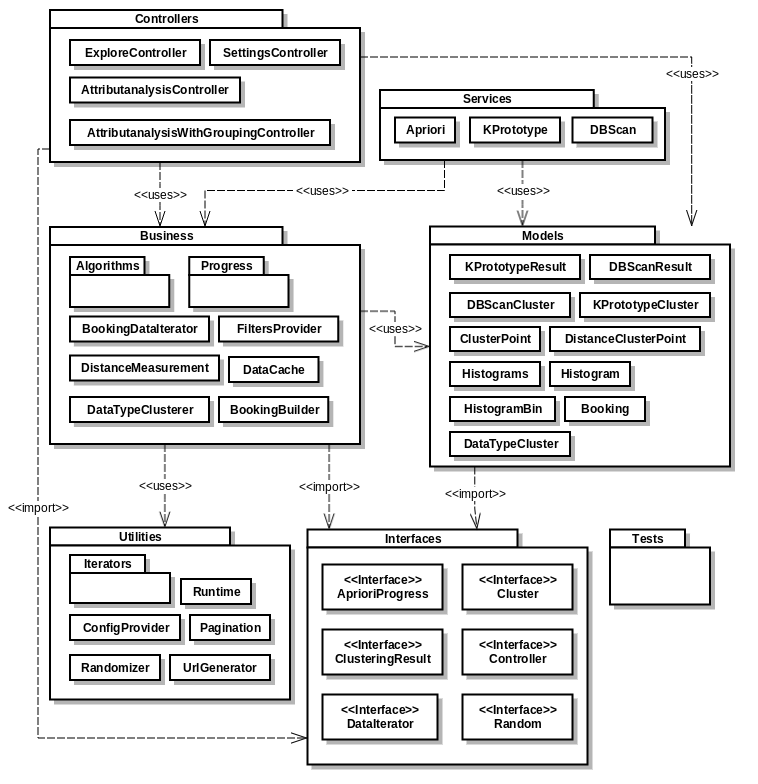
\includegraphics[width=1\textwidth]{images/diagram-package-diagram}
	\caption{Package-Struktur}
	\label{fig:proofofconcept:packagestruktur:1}
\end{figure}

Das Ziel war es, gemäss dem \gls{srp} eine starke Kohäsion und eine lose Kopplung zu erreichen. Deshalb wurde die Struktur der Packages ist so ausgelegt, dass die Abhängigkeiten von oben nach unten fliessen. Sprich ein oberes Packet kann ein unteres verwenden, jedoch nicht umgekehrt. Einstiegspunkte für die Ausführung des Programmes sind die Klassen in den Packages Controllers und Services. Ersteres wird vom Benutzer verwendet wenn er eine Seite angezeigt haben möchte. Die Services sind für die Hintergrundprozesse verantwortlich und führen eine Analyse der verschiedenen Algorithmen durch (siehe \cref{sec:proofofconcept:architektur:services} \nameref{sec:proofofconcept:architektur:services}). Nachfolgend werden die einzelnen Packages erklärt.

\begin{itemize}
	\item Controllers: Nehmen die Anfragen eines Benutzers entgegen und verarbeiten diese. Dazu verwenden sie Klassen aus dem Business welches ein Datenmodel zurückliefert. Dieses Model werden anschliessend vom Controller an die View übergeben welche die Ausgabe für den Browser generiert (siehe \cref{sec:proofofconcept:architektur:mvc} \nameref{sec:proofofconcept:architektur:mvc}).
	\item Services: Führen die verschiedenen Analysen durch. Sie sind so ausgelegt dass sie als eigenständiger Prozess im Hintergrund ausgeführt werden können (siehe \cref{sec:proofofconcept:architektur:services} \nameref{sec:proofofconcept:architektur:services}).
	\item Business: Beinhaltet die Geschäftlogik, was alles umfasst was mit den Models interagiert. Demnach die Algorithmen selber (im Unterpacket "`Algorithms"'), die Distanzmessung (Klasse DistanceMeasurement), den Datenzugriff (Klasse BookingDataIterator), etc. (siehe \cref{sec:proofofconcept:klassenstruktur:algorithmen} \nameref{sec:proofofconcept:klassenstruktur:algorithmen})
	\item Models: Klassen für die Datenhaltung welche möglichst wenig Logik beinhalten (siehe \cref{sec:proofofconcept:klassenstruktur:models} \nameref{sec:proofofconcept:klassenstruktur:models}).
	\item Utilities: Beinhalten Logik die nichts mit den Algorithmen zu tun hat und keine Models verwendet. Diese Klassen können für sich selber in einem anderen Projekt wiederverwendet werden.
	\item Interfaces: Alle verwendeten Interfaces.
	\item Tests: UnitTests (siehe \cref{sec:proofofconcept:unittests} \nameref{sec:proofofconcept:unittests}).
\end{itemize}

\subsection{Klassenstruktur}
\label{sec:proofofconcept:klassenstruktur}
Um den Aufbau der Lösung zu erklären werden die in diesem Abschnitt die Klassen sowie deren Abhängigkeiten gezeigt. Verwendet werden \gls{uml} Klassendiagramme für die Darstellung. Diese wurden jedoch in den \cref{app:klassendiagram} verschoben da sie wegen ihrer Grösse die Übersichtlichkeit erschweren.

Einige Klassen sind grün eingefärbt und stellen den Ausgangspunkte dar, von welchen die Erklärungen beginnen. Rot hinterlegt sind jene Klassen die von einer externen Bibliothek bereitgestellt werden.

Die Klasse ConfigProvider liefert die Konfigurationen und wird von vielen Klassen verwendet. Um die Übersichtlichkeit nicht unnötig zu erschweren wurde diese Abhängigkeit in den Klassendiagrammen weggelassen. 

\subsubsection{Models}
\label{sec:proofofconcept:klassenstruktur:models}
Die Models sind Datencontainer mit möglichst wenig Logik. 

\paragraph{Filter \& Felder} In \cref{fig:proofofconcept:klassenstruktur:5} werden die Filter und Felder gezeigt. Felder (Field) werden von den Algorithmen verwendet (z.B. Distanzmessung bei beim Clustering oder Häufigkeitszählung beim Apriori) sowie von den Filtern. Letztere werden benutzt um die Datenbasis einzuschränken. Es gibt verschiedene Arten von Feldern, welche direkt im Klassendiagram abgebildet sind. Dies wären zum Beispiel Fliesskommazahlen (FloatField), Ganzzahlen (IntegerField), Texten (String), etc. Welche Felder in der Datenbasis auf welchen Feldtypen im Code zugeordnet werden ist in der Konfiguration des Programmes definiert (siehe \cref{sec:proofofconcept:konfiguration} \nameref{sec:proofofconcept:konfiguration}).

\paragraph{Resultat des Apriori-Algorithmus} In \cref{fig:proofofconcept:klassenstruktur:6} werden die Histogramme abgebildet, welche üblicherweise zur Darstellung von Häufigkeitsverteilung verwendet wird. In dieser Arbeit werden sie für die Repräsentation des Resultates eines Apriori Algorithmuses benutzt. 
Ein "`Histograms"' besitzt ein oder mehrere "`Histogram"' welches wiederum ein oder mehrere "`HistogramBins"' enthält. "`Histograms"' beinhaltet sämtliche Attributmengen und stehen somit für das gesamte Resultat der Anaylse. Ein "`Histogram"' repräsentiert eine Iteration des Apriori Algorithmus (z.B. alle häufigen 2-Attributmengen). Schlussendlich enthält ein "`HistogramBin"' eine Attributkombination mit der Häufigkeit, wie oft sie in der Datenmenge vorkommt. Um dies an einem Beispiel zu zeigen wird eine "`Histograms"' hier gezeigt:
\begin{itemize}
\item \textbf{\#1 Histograms}:
	\begin{itemize}
		\item \textbf{\#1 Histogram}:
			\begin{itemize}
				\item \textbf{\#1 HistogramBin}: ((Distanz zum See = 200), 200/350 Buchungen)
				\item \textbf{\#2 HistogramBin}: ((Land = Schweiz), 150/350 Buchungen)
				\item \textbf{\#3 HistogramBin}: ((Jazzuci vorhanden = Ja), 75/350 Buchungen)
			\end{itemize}  
		\item \#2 Histogram:
			\begin{itemize}
				\item \textbf{\#1 HistogramBin}: ((Distanz zum See = 200, Land = Schweiz), 130/350 Buchungen)
				\item \textbf{\#2 HistogramBin}: ((Land = Schweiz, Jazzuci vorhanden = Ja), 70/350 Buchungen)
			\end{itemize}  
		\item \#3 Histogram:
			\begin{itemize}
				\item \textbf{\#1 HistogramBin}: ((Distanz zum See = 200, Land = Schweiz, Jazzuci vorhanden = Ja), 50/350 Buchungen)
			\end{itemize}  
	\end{itemize}  
\end{itemize}  


\paragraph{Resultat der Clustering-Algorithmen} Das Model für die Resultate der Clustering Algorithmen wird in \cref{fig:proofofconcept:klassenstruktur:7} gezeigt. Gemeinsamkeiten der beiden Algorithmen sind in den Interfaces "`ClusteringResult"' und "`Cluster"' zu finden. Deren Unterschiede sind jeweils in den entsprechenden Implementationen definiert. Die einzelnen Klassen werden nachfolgend beschrieben.
\begin{itemize}
	\item ClusterinResult: Definiert das ein Resultat vom DBScan und vom KProtoype ein oder mehrere Cluster besitzen muss.
	\begin{itemize}  
		\item DBScanResult: Das Resultat einer DBScan Analyse. Zusätzlich zu den Clustern selber besitzt die Klasse Noise-Punkte, welche keinem Cluster zugewiesen werden können (siehe \cref{sec:recherche:algorithmen:dbscan} \nameref{sec:recherche:algorithmen:dbscan}).
		\item KPrototypeResult: Das Resultat einer KPrototype Analyse. Neben den Clustern beinhaltet die Klasse die Gesamtkosten des Clusterings.
	\end{itemize}  
	\item Cluster: Ein Cluster besteht bei beiden Algorithmen aus einem oder mehreren Punkten.
		\begin{itemize}  
			\item DBScanCluster \& ClusterPoint: Der "`DBScanCluster"' besitzt nur die einzelnen Datenpunkte "`ClusterPoint"'. Diese beinhalten die ID der Buchung welche sie darstellen.
			\item KPrototypeCluster \& DistanceClusterPoint: Die Cluster beim KPrototypeCluster besitzen ein Zentrum, welches auf der Klasse "`KPrototypeCluster"' abgelegt ist. Jeder Datenpunkt in diesem Cluster ist vom Typ "`DistanceClusterPoint"' welcher neben der ID der Buchung welche er repräsentiert noch die Distanz bis zum Zentrum des Clusters beinhalten.
		\end{itemize}  
\end{itemize}  

%Grundelement ist das Interface "`ClusteringResult"', welches von "`DBScanResult"' und "`KPrototypeResult"' implementiert werden. Beide Klassen besitzen mehrere "`Cluster"'. Das "`DBScanResult"' besitzt jedoch noch Noise-Punkte und das "`KPrototypeResult"' der Gesamtfehler eines Clusters zu dessen Zentrum. 


\subsubsection{Controllers}
\label{sec:proofofconcept:klassenstruktur:controllers}
Die erste Abbildung \cref{fig:proofofconcept:klassenstruktur:1} zeigt die Controllers. 
\begin{itemize}
	 \item Controller: Das "`Controller"' Interface gibt eine "`run"' Methode vor welche den Inhalt zurück liefern welcher an den Browser zurückgesendet wird. Verwendet werden die Klassen für die Behandlung der einzelnen Internetseiten die dem Benutzer angezeigt werden können. Es gibt 4 Klassen welches dieses Interface implementieren.
	 \begin{itemize}
		\item ExplorerController: Ist für die Darstellung der Seite "`Einsehen der Stammdaten"' verantwortlich, welche in \cref{fig:konzept:mockups:stammdaten} abgebildet ist.
			\begin{itemize}
				\item BookingsProvider: Um die Buchungen zu laden wird der "`BookingsProvider"' verwendet. Dieser hat eine "`getSubset"' Methode mit welcher man sich die aktuelle Seite zurückgeben lassen kann. Er übernimmt nur die Aufgabe für die Unterteilung der Buchungen auf Seiten. Das Laden der Buchungen wird vom "`BookingDataIterator"' erledigt.
				\item BookingDataIterator: Wird in \cref{fig:proofofconcept:klassenstruktur:2} erläutert.
				\item UrlGenerator: Der URLGenerator wird benötigt um die Links zwischen den Seiten (Buchungslisten) zu erzeugen.
			\end{itemize}
		\item AttributanalysisController \& AttributanalysisWithGroupingController: Diese beiden Controller sind für die Darstellung von \cref{fig:konzept:mockups:apriori} und \cref{fig:konzept:mockups:clustering} verantwortlich und stossen die Services für die Analysen an (siehe \cref{sec:proofofconcept:architektur:services} \nameref{sec:proofofconcept:architektur:services}). 
		\item SettingsController: Zeigt ein Formular mit welchem die Einstellungen des Programmes angepasst werden können.
		\item Twig\_Environment: Dies ist die View (siehe \cref{sec:proofofconcept:architektur:mvc} \nameref{sec:proofofconcept:architektur:mvc}) welche das \gls{html} generiert, welches an den Browser gesendet wird für die Darstellung. Verwendet wird diese Klasse von allen Controllern.
		\item FiltersProvider: Liefert die Filter welche für den Aufbau des Formulares für die Einschränkung des Datenbestandes benötigt wird.
			\begin{itemize}
				\item DataTypeClusterer: Wird in \cref{fig:proofofconcept:klassenstruktur:2} erläutert.
			\end{itemize}
	 \end{itemize}
\end{itemize}

\subsubsection{Algorithmen}
\label{sec:proofofconcept:klassenstruktur:algorithmen}
\cref{fig:proofofconcept:klassenstruktur:2} zeigt den Service für den Apriori Algorithmus.
\begin{itemize}
	\item AprioriAlgorithm: Führt den Apriori Algorithmus aus. Abhängig was der Klasse übergeben wird analysiert sie die gesamten Datenbasis, eine durch Filter eingeschränkten Untermenge, oder das Resultat eines Clusterings. Gesteuert wird dies über den "`DataIterator"' und den "`AprioriProgress"' welche nachfolgend beschrieben werden.
	\item AprioriProgress: Speichert das Resultat der Apriori Analyse. 
	\begin{itemize}
		\item AprioriProgressToFile: Speichert das Resultat der Apriori Analyse in ein File ab. Diese Klasse wird verwendet wenn der Algorithmus auf der gesamten Datenbasis (oder auf einer durch Filter eingeschränkten Untermenge) durchgeführt wird. 
		\item AprioriProgressForCluster: Wenn der Apriori Algorithmus das Resultat eines Clusterings analysiert kann diese Klasse verwendet werden. Sie speichert das gesamte Ergebnis ab. Sprich es müssen alle Cluster sowie deren jeweiligen Resultate des Apriori-Algorithmus übergeben werden.
	\end{itemize}
	\item BookingDataIterator: Diese Klasse implementiert das Iterator-\gls{pattern}. Sie ermöglicht es Buchung für Buchung eine Datenquelle zu durchlaufen. Intern wird ein "`DataIterator"' verwendet um auf die Quelle der Daten zuzugreifen. Dieser liefert ein unstrukturiertes Array zurück, welches der "`BookingDataIterator"' in eine Buchung umwandelt.
		\begin{itemize}
			\item Iterator \& DataIterator: Von \gls{php} wird für die Implementierung des Iterator-\gls{pattern} ein Iterator Interface zur Verfügung gestellt. Das "`DataIterator"' Interface erweitert jenes von \gls{php} um eine Methode "`skip"', mit welcher eine Anzahl an Zeilen in der Datenquelle übersprungen werden kann (wird vom "`ExploreController"' verwendet), sowie eine Funktion "`count"', welche die gesamte Anzahl an Resultaten zurück gibt. Es gibt 4 Iteratoren, welche das "`DataIterator"' Interface implementieren. Die Auswahl des geeigneten Iterators wird im \cref{sec:proofofconcept:performance} \nameref{sec:proofofconcept:performance} erläutert.
				\begin{itemize}
					\item LoadRedisDataIterator \& Redis: Der "`LoadRedisDataIterator"' lädt die Daten aus einer Redis InMemory Datenbank. Verwendet wird dazu die "`Redis"' Klasse aus der \gls{pecl} (siehe \cref{sec:proofofconcept:externebibliotheken:redis} \nameref{sec:proofofconcept:externebibliotheken:redis} für Details zu Redis).
					\item LoadIncrementalCSVDataIterator: Lädt die Daten aus einer \gls{csv}-Datei. Jede Zeile wird einzeln aus dem File gelesen.
					\item LoadAllCSVDataIterator: Lädt die Daten aus einer \gls{csv}-Datei. Zu Beginn werden alle Zeilen ins Memory des Programmes geladen, aus welchem Zeile für Zeile zurückgegeben wird.
					\item LoadClusterDataIterator: Der Klasse muss ein Cluster übergeben werden, über welchen iteriert wird. Verwendet wird der "`LoadClusterDataIterator"' für die Apriori-Analyse nachdem ein Clustering durchgeführt wurde.
				\end{itemize}
			\item DataTypeClusterer: Er übernimmt ein Array an Feldern mit untypisierten Daten aus einer Datenquelle oder den Filtern, typisiert diese und gruppiert sie. Beispiel an Daten die an den "`DataTypeClusterer"' übergeben werden:
			\begin{lstlisting}[language=php]
var $\textdollar$rawData = array(
	'distanceToPublicTransport' => 400
	'distanceToSea' => 200
	'country' => 'Switzerland'
)
			\end{lstlisting}
			Dabei handelt es sich um ein Array mit 3 Feldern. Der DataTypeClusterer wandelt die 2 Distanzfelder in Objekte vom Typen "`DistanceField"' um und gruppiert sie zusammen unter "`distanceFields"'. Das Land (country) wird in ein "`StringField"' Ojekt umgewandelt und unter "`stringFields"' gruppiert. Das Resultat sieht das etwas vereinfacht so aus:
			\begin{lstlisting}[language=php]
object(DataTypeCluster) {
	"distanceFields": array(
		object(DistanceField) {
			"name" => string("distanceToPublicTransport")
			"value" => int(400)
		},
		object(DistanceField) {
			"name" => string("distanceToPublicTransport")
			"value" => int(400)
		},
	),
	"stringFields": array(
		object(StringField) {
			"name" => string("country")
			"value" => string("Switzerland")
		}
	)
}
			\end{lstlisting}
			\item BookingBuilder: Erstellt ein Objekt "`Booking"' mit hilfe eines "`DataTypeClusterer"' aus einem unstrukturierem Array.
		\end{itemize}
\end{itemize}

\cref{fig:proofofconcept:klassenstruktur:3} zeigt den Service für den DBScan Algorithmus. Die Klasse "`BookingDataIterator"' wurde bereits im \cref{fig:proofofconcept:klassenstruktur:2} erläutert und wurde deshalb nicht mehr detailliert abgebildet.
\begin{itemize}
	\item DBScanAlgorithm: Führt den DBScan Algorithmus aus. 
	\item ClusteringProgress \& DBScanClusteringProgress: Eine abstrakte Klasse welche das Resultat eines Clusterings in ein File abspeichert. Kann für den DBScan und den KPrototype verwendet werden. Die abgeleitete Klasse "`DBScanClusteringProgress"' wird lediglich benötigt um die richtige View zu laden und die korrekte Konfiguration bereitzustellen.
	\begin{itemize}
		\item Runtime: Verfolgt die Laufzeit des Algorithmus seit der Service gestartet wurde. 
	\end{itemize}
	\item DistanceMeasurement: Implementation der Distanzmessung aus der \cref{eq:recherche:clusteranalysis:2}.
\end{itemize}

\cref{fig:proofofconcept:klassenstruktur:4} zeigt den Service für den KPrototype Algorithmus. Die Klassen "`BookingDataIterator"' und "`DistanceMeasurement"' wurden bereits dokumentiert und werden hier nicht mehr erläutert.
\begin{itemize}
	\item KPrototypeAlgorithm: Führt den KPrototype Algorithmus aus. 
	\item ClusteringProgress \& KPrototypeClusteringProgress: Der ClusteringProgress ist der selbe wie in \cref{fig:proofofconcept:klassenstruktur:3}. Die abgeleitete Klasse "`KPrototypeClusteringProgress"' liefert, gleich wie "`DBScanClusteringProgress"' die View sowie die Konfiguration. 
	\item Random, Randomizer, Redis \& BookingBuilder: Der KPrototype Algorithmus wählt die initialen Clusterzentren zufällig. Dafür werden diese 4 Klassen benötigt. Random und Randomizer erlauben es zufällg eine Buchungs-Id auszuwählen. Die Redis InMemory Datenbank liefert die Rohdaten der Buchung und der "`BookingBuilder"' wandelt sie in eine Klasse "`Booking"' um (siehe \cref{sec:proofofconcept:externebibliotheken:redis} \nameref{sec:proofofconcept:externebibliotheken:redis} für Details zu Redis).
\end{itemize}

\section{Abläufe}
Zuerst wird der Kommunikationsablauf zwischen dem Benutzer, dem Server und der Hintergrundprozesse erläutert. Der \cref{sec:proofofconcept:kommunikationsablauf} geht dann auf die einzelnen Punkte im Kommunikationsablauf genauer ein und erläutert diese mit der Unterstützung von \gls{uml}-Sequenzdiagrammen.

\subsection{Kommunikationsablauf}
\label{sec:proofofconcept:kommunikationsablauf}
In \cref{fig:proofofconcept:kommunikationsablauf:1} wird der Kommunikationsablauf aufgezeigt, welcher zwischen dem Webserver und dem Browser des Benutzers stattfindet. Massgeblich beeinflusst wurde der Ablauf durch die Algorithmen (siehe \cref{sec:proofofconcept:architektur:anforderungen:algorithmen} \nameref{sec:proofofconcept:architektur:anforderungen:algorithmen}). Sobald der Benutzer eine Analyse startet wird eine Anfrage an den Server gestellt. Dieser erstellt einen Hintergrundprozess welcher die Analyse durchführt und gibt danach direkt eine Antwort an den User zurück. 

Der Hintergrundprozess führt die Analyse durch und schreibt periodisch einen Zwischenstand im \gls{html}-Format in eine Datei.

Sobald die Analyse vom Server angestossen wurde kann dieser eine Rückmeldung zum Benutzer senden mit der Nachricht, dass die Analyse gestartet wurde. Der Browser des User beginnt darauf hin, die \gls{html}-Datei auf dem Server nach dem Zwischenstand abzufragen bis die Analyse beendet ist.
\begin{figure}[H]
	\RawFloats
	\centering
	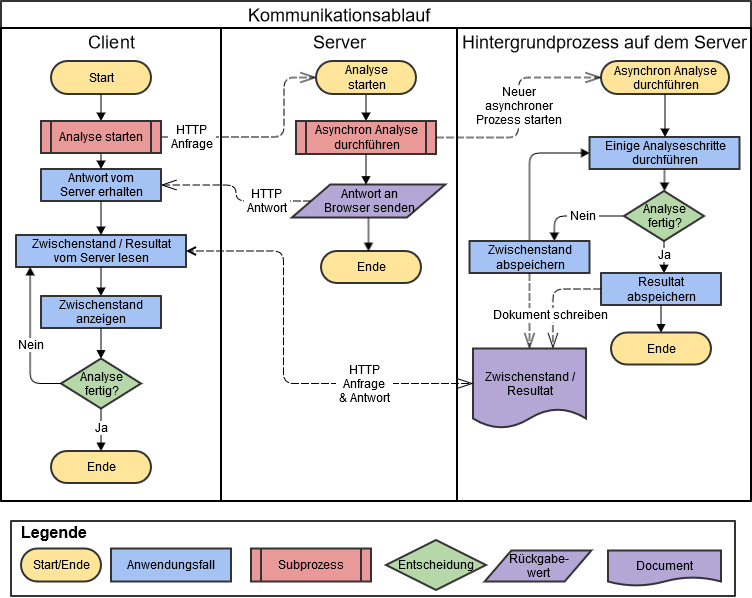
\includegraphics[width=1\textwidth]{images/diagram-communication-flow}
	\caption{Kommunikationsablauf}
	\label{fig:proofofconcept:kommunikationsablauf:1}
\end{figure}



\subsection{Programmablauf}
\label{sec:proofofconcept:programmablauf}
Im \cref{sec:proofofconcept:kommunikationsablauf} wurde der Ablauf zwischen dem Benutzer und dem Server illustriert. Hier werden die Abläufe auf dem Webserver sowie der Hintergrundprozesse erläutert.

\subsubsection{Webserver}
\label{sec:proofofconcept:architektur:webserver}
Der Webserver nimmt einen Request des Users entgegen und verarbeitet diesen. Der Ablauf wird in \cref{fig:proofofconcept:architektur:webserver:1} visualisiert.

\begin{figure}[H]
	\centering
	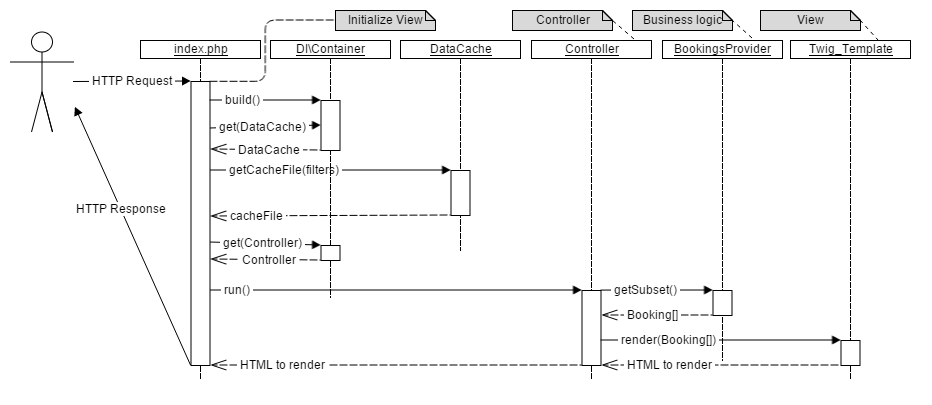
\includegraphics[width=1\textwidth]{images/diagram-sequence-controllers}
	\caption{Sequenzdiagramm für den Ablauf einer "`Explore"'-Anfrage}
	\label{fig:proofofconcept:architektur:webserver:1}
\end{figure}

Aufgerufen wird stets die Datei "`index.php"'. Diese Initialisiert zuerst den dependency injection Container (siehe \cref{sec:proofofconcept:dependency-injection} \nameref{sec:proofofconcept:dependency-injection}) und zwischenspeichert die Datenquelle für die vom Benutzer übergebenen Filterkriterien (siehe \cref{sec:proofofconcept:performance:caching} \nameref{sec:proofofconcept:performance:caching}).

Danach wird der Controller aufgerufen welcher den Request des Benutzers behandelt. Der Controller führt die Geschäftslogik aus (im obigen Beispiel ist dies die Klasse "`BookingsProvider"') und übergibt das Resultat an die View welche für die Darstellung der Daten zuständig ist. Der Rückgabewert wird dem Benutzer im Browser angezeigt.

Dieser Ablauf ist gültig für die "`Explore"'-Ansicht, auf welcher der User die Buchungen einsehen kann. Wenn ein Algorithmus ausgeführt werden soll fällt die Geschäftslogik weg und es wird stattdessen ein Hintergrundprozess gestartet, welcher diese ausführt.

\subsubsection{Services}
\label{sec:proofofconcept:architektur:services}
Services sind Hintergrundprozesse welche die Implementation der Algorithmen ausführen. Diese sind nötig um die Laufzeitlimite von Prozessen in einem Webserver zu umgehen. Weitere Informationen hierzu werden im \cref{sec:proofofconcept:kommunikationsablauf} gegeben.

Dieser Abschnitt erklärt die Abläufe der Services und wie sie angestossen werden. Für die Darstellung werden \gls{uml} Sequenzdiagramme verwendet. Die Implementation der Algorithmen selber wird hier nicht genauer beschrieben. Zum einen sind diese im \cref{sec:recherche:algorithmen} bereits dokumentiert und wurden hier entsprechend umgesetzt. Zum anderen würde ein Sequenzdiagramm der Algorithmen zu gross ausfallen und deshalb nicht zum Verständnis beitragen können.


\paragraph{Anstossen der Services}
Die Services werden von den Controllern angestossen. Es wird ein Kommandozeilen-Befehl ausgeführt welcher im folgender Ansicht beispielhaft am Apriori-Algorithmus aufgezeigt wird.

\blockquote[]{
php /Services/Apriori/apriori.php ``stars=4,country=Switzerland'' > /Services/Apriori/wip/output.txt 2>\&1 \& echo \$! > /pidfile.txt
}

Zur erklärung dieses Befehles wird er aufgebrochen:
\begin{itemize}
	\item \textbf{php}: Es wird der Befehl "`php"' ausgeführt welcher ein \gls{php} Programm startet.
	\item \textbf{/Services/Apriori/apriori.php}: Das auszuführende \gls{php} Programm. Hier die Apriori Analyse.
	\item \textbf{``stars=4,country=Switzerland''}: Parameter die an das "`apriori.php"' Programm übergeben werden. In diesem Beispiel sind das die Filterkriterien des Benutzers.
	\item \textbf{> /Services/Apriori/wip/output.txt}: Mit "`>"' wird die Standartausgabe des Programmes definiert. Jegliche Ausgabe des Programmes wird hiermit in die Datei "`output.txt"' geschrieben.
	\item \textbf{2>\&1}: Mit "`2>"' wird gesagt wohin Fehlemeldungen geschrieben werden. \&1 gibt an dass es an den selben Ort wie die Standartausgabe gespeichert werden soll. Also auch ins "`output.txt"'.
	\item \textbf{\&}: Durch das \& wird der Befehl im Hintergrund ausgeführt. Wenn dies nicht angegeben wird würde das Programm, welches den "`php"' Befehl gestartet hat warten, bis das "`apriori.php"' Programm fertig gearbeitet hat.
	\item \textbf{echo \$! > /pidfile.txt}: "echo \$!" gibt die Prozessid des "`apriori.php"' Programmes aus. Mit "`> /pidfile.txt"' wird die Ausgabe (also die Prozessid) in die Datei "`pidfile.txt"' geschrieben.
\end{itemize}

\paragraph{Ablauf des Apriori-Programmes}
Der Ablauf der Apriori-Analyse wird in \cref{fig:proofofconcept:architektur:hintergrundprozesser:1} verbildlicht.

\begin{figure}[H]
	\centering
	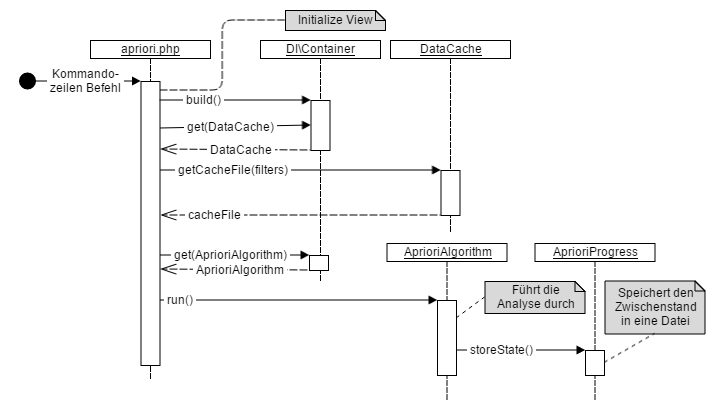
\includegraphics[width=1\textwidth]{images/diagram-sequence-apriori}
	\caption{Sequenzdiagramm für die Initialisierung der Apriori-Analyse}
	\label{fig:proofofconcept:architektur:hintergrundprozesser:1}
\end{figure}

Der Anfang mit dem Erstellen des "`Container"' und dem Caching ist gleich wie in \cref{fig:proofofconcept:architektur:webserver:1}. Das "`apriori.php"' Programm ruft danach den Apriori-Algorithmus auf welcher sein Resultat periodisch in eine Datei schreibt (siehe \cref{sec:proofofconcept:kommunikationsablauf} \nameref{sec:proofofconcept:kommunikationsablauf}). Dies ermöglicht dem Algorithmus regelmässig einen Zwischenstand abzuspeichern welcher dem Benutzer angezeigt werden kann.

\paragraph{Ablauf des Clustering-Programmes}
Der Ablauf der Clustering-Analysen ist identisch zu jenem des Apriori-Algorithmus, mit zwei Ausnahmen. Zum einen wird vor dem "`AprioriAlgorithm"' der "`KPrototypeAlgorithm"' ausgeführt wird, welcher ein "`KPrototypeResult"' zurück liefert. 
Zum anderen wird dem "`AprioriAlgorithm"' das Resultat vom KPrototype als Parameter übergeben. Dadurch ist em dem "`KPrototypeAlgorithm"' möglich, nur die Elemente eines Clusters zu analysieren und nicht die gesamte Datenmenge. 
Es wurde bewusst entschieden, dass der "`AprioriAlgorithm"' aus der kprototype.php Datei hinaus aufgerufen wird. Dadurch kann zukünftig dieser Algorithmus einfach durch eine Alternative ausgetauscht werden.
Abgebildet ist der Ablauf in \cref{fig:proofofconcept:architektur:hintergrundprozesser:2}. 
\begin{figure}[H]
	\centering
	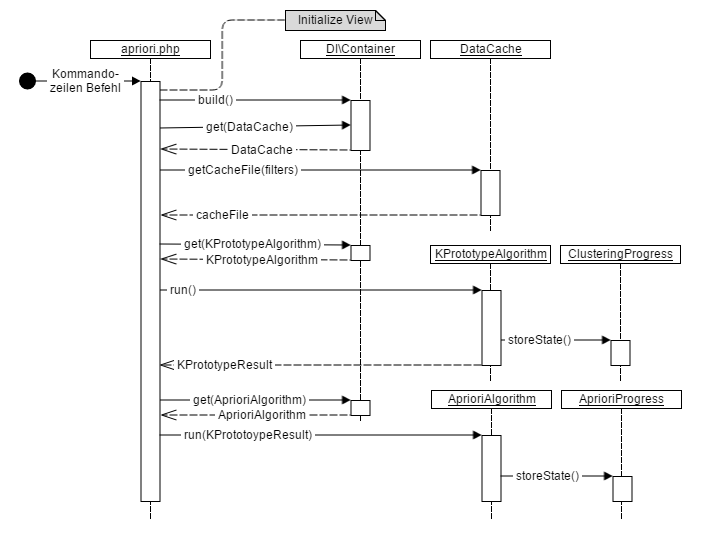
\includegraphics[width=1\textwidth]{images/diagram-sequence-kprototype}
	\caption{Sequenzdiagramm für die Initialisierung der KPrototype-Analyse}
	\label{fig:proofofconcept:architektur:hintergrundprozesser:2}
\end{figure}

Auf ein Sequenzdiagramm für den DBSCAN-Algorithmus wird hier verzichtet, denn die Visualisierung des DBSCAN-Ablaufs ist identisch wie jener vom KPrototype. Lediglich die Namen der aufgerufenen Klassen müssten angepasst werden.


\section{Performance}
\label{sec:proofofconcept:performance}
Da die Geschwindigkeit kritisch ist wenn man mit einer grossen Datenmenge arbeitet, wurde ein Caching eingesetzt sowie mehrere Varianten für das Laden der Daten evaluiert. Diese Themen werden nachfolgend beschrieben.

\subsection{Datenzugriff}
\label{sec:proofofconcept:performance:datenzugriff}
Das Laden der Daten ist kritisch für die Geschwindigkeit des Gesamtsystemes. Im speziellen für die Clustering Algorithmen, da dort mehrfach über die gesamte Datenbasis iteriert werden muss. Deshalb wurden verschiedene Möglichkeiten in Betracht gezogen.

Da die Datenbasis im \gls{csv}-Format vorliegt wurden zwei Varianten für den Datenzugriff eruiert. Mit \gls{php} kann entweder Zeile für Zeile aus einer Datei gelesen werden, oder alles zusammen.  Bei der ersten Version wird eine Zeile erst geladen, wenn diese angefragt wird. Bei der zweiten werden alle Einträge aus der Datei in den Arbeitsspeicher gelesen und zur Laufzeit darüber iteriert.

Mit der Redis InMemory Datenbank gibt es eine dritte Möglichkeit wie auf die Daten zugegriffen werden kann (siehe \cref{sec:proofofconcept:externebibliotheken:redis} \nameref{sec:proofofconcept:externebibliotheken:redis}). Hierzu müssen die Daten zuerst in die Redis Datenbank importiert werden und können dann bei der Analyse nur noch abgefragt werden. Dazu wurde ein Hilfsprogramm erstellt welches die Daten aus dem \gls{csv}-File ausliest nach Redis importiert. Der Quellcode kann unter \url{https://github.com/soultemptation/bookinganalyzerimpl/blob/master/Services/FillRedis/fillredis.php} eingesehen werden.

Für die drei Herangehensweisen wurde jeweils ein Iteratoren erstellt (siehe \cref{sec:proofofconcept:klassenstruktur:algorithmen} \nameref{sec:proofofconcept:klassenstruktur:algorithmen}) um die Geschwindigkeit zu vergleichen. Dazu wurde die Apriori Analyse auf allen Daten fünf mal ausgeführt und der Durchschnitt genommen.

\begin{itemize}
	\item Version 1, Zeile für Zeile laden: 9.82 Sekunden
	\item Version 2, Alles in den Zwischenspeicher laden: 10.62 Sekunden
	\item Version 3, Daten aus Redis laden: 23.10 Sekunden
\end{itemize}

Die Variante mit dem Laden Zeile für Zeile ist mit der durchschnittlichen Zeit von 9.82 am schnellsten. Dies ist überraschend, da zu erwarten war dass auf die Daten schneller zugegriffen werden kann wenn sie im Zwischenspeicher gelagert werden. Vor allem das Resultat mit Redis war verblüffend, da sie doppelt so lange dauert, obwohl die Daten vorher schon in der Datenbank vorhanden sein müssen.

\subsection{Caching}
\label{sec:proofofconcept:performance:caching}
Im \cref{sec:proofofconcept:performance:datenzugriff} wurde die Wichtigkeit des Datenzugriff erläutert. Dieser kann durch ein Caching (Zwischenspeichern der Daten) nochmals beschleunigt werden. 

Um dies zu zeigen wurde ein Test gemacht mit der Ansicht, in welcher die Daten eingesehen werden können. Es sollen alle Buchungen von Objekten mit einer 1 Sterne-Bewertung angezeigt werden. Mit einem Caching dauert es durchschnittlich 0.31 Sekunden um die letzten 30 Instanzen anzuzeigen (wenn der Cache vorgewärmt ist, mehr dazu weiter unten). Ohne Caching hingegen benötigt das Programm durchschnittlich 10.24 Sekunden. Dies ist eine Verbesserung um das 33-fache.

Dieses Beispiel ist ein Extremfall, da es nur 1'548 Buchungen von 1 Sterne Objekten in der gesamten Datenbasis gibt. Je mehr Buchungen herausfiltert werden, desto bessere Ergebnisse liefert das Caching.

Wenn die ersten 30 Buchungen in der Buchungen-Einsehen Ansicht angezeigt werden, wird eine Cache-Datei geschrieben welche nur jene Instanzen enthalten, die auf die filterkriterien passen. Dazu wird die gesamte Datenbasis durchlaufen und die Kriterien auf jede Buchung anzuwenden. Sobald dies geschehen ist gilt der Cache für diese Kriterien als "`vorgewärmt"'. 
Dieses aufwärmen dauert durchschnittlich 10 Sekunden. Dies ist die Zeit welche die Anfrage im Beispiel oben ohne Caching benötigt hat. 

Der Vorteil des Cachings ist es, dass Filterkriterien für eine Anfrage nur einmal angewendet werden müssen. Im Beispiel oben müsste ohne Caching alle 111'442 Buchungen durchlaufen und die Kriterien angewendet werden, um die letzten 30 der 1'548 Buchungen anzuzeigen. Durch den Zwischenspeicher kann dass Programm direkt zu den letzten 30 Instanzen iterieren und diese anzeigen. Deshalb liefert das Caching bessere Ergebnisse, wenn mehr Daten durch das Filtrieren wegfallen.

Das Caching übernimmt die Klasse "`DataCache"' (siehe \cref{sec:proofofconcept:packagestruktur} \nameref{sec:proofofconcept:packagestruktur}). Wie der Cache in den Programmablauf eingebunden wird ist in den Squenzdiagrammen im \cref{sec:proofofconcept:programmablauf} \nameref{sec:proofofconcept:programmablauf} beschrieben.

\section{Externe Bibliotheken}
\label{sec:proofofconcept:externebibliotheken}
Dieser Abschnitt erläutert welche externe Bibliotheken eingesetzt wurden.

\subsection{Dependency Injection mit PHP-DI}
\label{sec:proofofconcept:dependency-injection}
% und um die Entkoppelung der einzelnen Module zu ermöglichen ein Dependency Injection Framework verwendet. Diese und weitere Punkte werden nachfolgend beschrieben.
Bei der Dependency Injection handelt es sich um ein \gls{pattern}
das zum Ziel hat, eine möglichst niedrige Kopplung zu erreichen. Dies bedeutet, dass eine Klasse so wenig Abhängigkeiten wie möglich zu anderen Komponenten aufweisen soll. Dadurch können einzelne Klassen einfacher ausgetauscht werden washt die Wartbarkeit des Systems erhöht sowie die Leserlichkeit des Codes fordert. Dies soll anhand eines Beispieles aufgezeigt werden.

\begin{lstlisting}[language=php]
var _x = $\textdollar$y
\end{lstlisting}

\begin{lstlisting}[language=php]
class Car {
	public $\textdollar$engine;
	
	public function __construct() {
		$\textdollar$this->engine = new V6Engine();
	}
	
	public function accelerate() {
		$\textdollar$this->engine->accelerate();
	}
}
\end{lstlisting}

Im obigen Code wird eine Klasse Car erstellt in dessen Konstruktor ein V6 Motor instanziiert  wird. Der Code ist jetzt direkt gekoppelt mit der Klasse V6Engine. Wenn ein Auto mit einem V4Engine erstellt werden soll muss die Klasse entsprechend angepasst werden. 


\begin{lstlisting}[language=php]
class Car {
	public $\textdollar$engine;
	
	public function __construct(Engine engine) {
		$\textdollar$this->engine = engine;
	}
	
	public function accelerate() {
		$\textdollar$this->engine->accelerate();
	}
}
\end{lstlisting}

Hier wurde die Klasse so angepasst, dass der Konstruktor keinen Motor erstellt, sondern diesen über die Parameter übernimmt. So kann von aussen gesteuert werden, welchen Engine das Auto beinhaltet. 

In der Arbeit werden alle Komponenten über Dependency Injection in Klassen hineingereicht. Die einzige Ausnahme sind die Models, weshalb sie auch möglichst wenig Logik beinhalten sollten (siehe \cref{sec:proofofconcept:packagestruktur} \nameref{sec:proofofconcept:packagestruktur}). Dies kann besonders gut mit den Iteratoren veranschaulicht werden. Die Klasse "`BookingDataIterator"' nimmt ein Interface "`DataIterator"' entgegen. Es gibt 5 Klassen welche dieses Interface implementieren wovon 3 hier erläutert werden:
\begin{itemize}
	\item LoadAllCsvDataIterator: Lädt alle Buchungsdaten aus einem File ins Memory und iteriert dann über die einzelnen Instanzen.
	\item LoadIncrementalCsvDataIterator: Lädt eine Instanz nach der anderen aus dem File.
	\item LoadRedisDataIterator: Lädt eine Instanz nach der anderen aus einer Redis Datenbank (In Memory Datenban) (siehe \cref{sec:proofofconcept:externebibliotheken:redis} \nameref{sec:proofofconcept:externebibliotheken:redis}).
\end{itemize}

Es gibt demnach 3 verschiedene Möglichkeiten, wie auf die Daten zugegriffen werden kann. Mittels Dependency Injection kann nun von aussen bestimmt werden, wie der "`BookingDataIterator"' auf die Daten zugreift.

Für das Dependency Injection \gls{pattern}
 wird das Framework PHP-DI verwendet (siehe \url{http://php-di.org/}). In der ersten geladenen Datei wird der gesamte Objektgraph aufgebaut. Dort wird bestimmt, welche Klasse in den "`BookingDataIterator"' übergeben wird. Ein Beispiel wird nachfolgend präsentiert:
 
\begin{lstlisting}[language=php]
$\textdollar$builder = new DI\ContainerBuilder();
$\textdollar$builder->addDefinitions([
    [...]
    DataIterator::class => DI\object(LoadIncrementalCsvDataIterator::class),
    [...]
]);
$\textdollar$container = $\textdollar$builder->build();
$\textdollar$apriori = $\textdollar$container->get('AprioriAlgorithm');
$\textdollar$apriori->run();
\end{lstlisting}

Zuerst wird ein "`ContainerBuilder"' erstellt. Auf diesem wird definiert, dass für das "`DataIterator"' Interface die Klasse "`LoadIncrementalCsvDataIterator"' verwendet werden soll. Danach wird auf Zeile 7 ein "`Container"' erstellt und anschliessend eine Instanz der Klasse "`AprioriAlgorithm"' angefordert. Der Container analysiert die Klasse und sieht dass ein "`DataIterator"' erwartet wird und reicht deshalb ein "`LoadIncrementalCsvDataIterator"' in den "`AprioriAlgorithm"' rein. Somit kann auf oberster Ebene gesteuert werden, welche Klassen wo übergeben werden.

\subsection{Frontend mit Twitter Bootstrap}
\label{sec:proofofconcept:externebibliotheken:bootstrap}
Für das Design des Webseite wurde Twitter Bootstrap (url{http://getbootstrap.com/})verwendet. Es bietet viele Komponenten welche man für die Entwicklung einer Webseite verwendet kann. Dies erleichtert die Umsetzung, da man sich keine Gedanken darüber machen muss wie die Seite aufgebaut oder gestaltet wird. 

Eingesetzt wurde folgende Komponenten:
\begin{itemize}
	\item Navigation: Die Navigation welche auf jeder Seite zuoberst dargestellt wird (\url{http://getbootstrap.com/components/#navbar}).
	\item Formulare: Die Formulare für die Einschränkung des Datenbestandes (\url{http://getbootstrap.com/css/#forms}).
	\item Tabellen: Für die Auflistung der Buchungen für das einsehen der Stammdaten sowie den Resultaten der Apriori Analyse. (\url{http://getbootstrap.com/css/#tables}).
	\item Pagination: Die Paginierung beim einsehen der Stammdaten (\url{http://getbootstrap.com/components/#pagination})
	\item Glyphicons: Die Icons für die Preise und das Häkchen der binären Attribute (\url{http://getbootstrap.com/components/#glyphicons}).
\end{itemize}

\subsection{JavaScript Framework mit JQuery}
Für die JavaScript Entwicklung wurde JQuery eingesetzt (\url{https://jquery.com/}). Verwendet wurde die Bibliothek für die Abfrage des Zwischenstandes einer Analyse vom Server. Für die Textvervollständigung bei der Eingabe der Destination wurde zusätzlich noch die JQuery Erweiterung "`Autocomplete"' eingesetzt (\url{https://jqueryui.com/autocomplete/}).

\subsection{Less mit Grunt}
Das Styling einer Webseite wird üblicherweise mit \gls{css} gemacht. Es gibt jedoch Erweiterungen dazu wie LESS oder SASS. In diesem Projekt wurde LESS eingesetzt (\url{http://lesscss.org/}). Dieses muss jedoch in \gls{css} umgewandelt werden wozu Grunt verwendet wurde. (\url{https://gruntjs.com/}).

\subsection{Templating mit Twig}
\label{sec:proofofconcept:externebibliotheken:twig}
\gls{html} Templates werden benutzt um die Logik des Programmes von der Darstellung zu trennen (siehe \cref{sec:proofofconcept:architektur:anforderungen:ansichten} \nameref{sec:proofofconcept:architektur:anforderungen:ansichten}). Dazu wurde die \gls{php} Template Bibliothek Twig eingesetzt (\url{https://twig.sensiolabs.org/}).

%"`"'
In der Umsetzung sind die Templates von Twig im Ordner "`Templates"' hinterlegt. Nachfolgend werden die Templates kurz erklärt.
\begin{itemize}
	\item base.twig: Beinhaltet das Grundgerüst der Webseite. Es bietet Platzhalter, welche durch andere Templates befüllt werden können (dazu mehr unter \url{https://twig.sensiolabs.org/doc/2.x/tags/block.html}).
	\item head.twig: Gibt den Kopfbereich der \gls{html}-Datei aus, welche zusätzliche Daten zur Webseite beinhaltet, die nicht zur Darstellung benötigt werden. Zum Beispiel den Namen der Seite, wer die Seite erstellt hat, welche Bildschirmgrössen unterstützt werden, etc.
	\item footer.twig: Gibt den Fussbereich der Seite aus. 
	\item navigation.twig: Gibt die Navigation aus, mit welcher zwischen den einzelnen Ansichten gewechselt werden kann.
	\item explore.twig: Stellt die Ansicht für das einsehen der Stammdaten zusammen. 
	\item attributanalysis.twig \& attributanalysisWithGrouping.twig: Diese Templates stellen die Grundgerüste für die Attributanalyse und die Attributanalyse mit Groupierung dar. Sie beinhalten die Filter sowie einen Platzhalter welcher durch die Services befüllt werden kann.
	\item settings.twig: Stellt die Ansicht für das anpassen der Einstellungen dar. 
	\item filters.twig: Gibt das Formular für die Filtrierung der Stammdaten aus.
	\item bookingListing.twig: Gibt die Stammdaten als Tabelle aus. Verwendet wird dies für das einsehen der Stammdaten.
	\item apriori.twig: Das Resultat oder der Zwischenstand der Apriori kann mit dem apriori.twig Template erstellt werden.
	\item kprototypeClusters: Gibt das Resultat oder den Zwischenstand des KPrototype Clusterings aus.
	\item dbscanClusters: Gibt das Resultat oder den Zwischenstand des DBScan Clusters aus.
	\item histogramsAsTable.twig: Dies gibt die Resultate des Apriori Algorithmus als Tabelle aus. 
\end{itemize}

\subsection{UnitTests mit PHPUnit}
\label{sec:proofofconcept:externebibliotheken:phpunit}
UnitTests wurden mit PHPUnit umgesetzt (\url{https://phpunit.de/}). Mehr dazu im \cref{sec:proofofconcept:unittests} \nameref{sec:proofofconcept:unittests}

\subsection{Package Managing mit Composer}
Ein Package Manager verwaltet die Abhängigkeiten von externen Bibliotheken welche in einem Projekt benutzt werden. In der Entwicklung dieser Arbeit wurde Composer (\url{https://getcomposer.org/}) eingesetzt. Verwendet wurde der Package Manager um Bibliotheken wie Twig, PHPUnit und PHP-DI zu verwalten.

Composer wird über die Konfigurationsdatei "`composer.json"' gesteuert. In diesem Projekt sind dort folgende Abhängigkeiten definiert:

\begin{lstlisting}[language=json]
  "require": {
    "twig/twig": "2.2.*",
    "twbs/bootstrap": "3.3.7",
    "phpunit/phpunit": "6.0.0",
    "php-di/php-di": "5.4.*",
    "mikey179/vfsStream": "1.6.*"
  }
\end{lstlisting}

Dadurch wird definiert, dass dieses Projekt abhängigkeiten zu Twig, Bootstrap, PHPUnit, PHP-DI und vfsStream besitzt. Daneben stehen jeweils die Versionen die benutzt werden sollen. Ein "`*"' bedeutet dass die Version nicht fix ist und das Updates automatisch installiert werden dürfen. Zum Beispiel soll für Twig die Version 2.2.* benutzt werden. Aktuell ist gerade die Version 2.2.0. Falls irgendwann 2.2.1 erscheint wird Composer diese Version installieren. Falls jedoch 2.3.0 veröffentlicht wird bleibt Composer bei der Version 2.2.0. 

Die Package die in der Datei "`composer.json"' definiert sind werden auf der Webseite \url{https://packagist.org} gesucht. Dort sind die Packete hinterlegt. Geht man auf diese Seite kann man nach dem Text "`twig/twig"' suchen und findet dort Details zu Twig, wie zum Beispiel wer es entwickelt, welche Version gerade aktuell ist und Abhängigkeiten die das Paket mit sich bringt.

Nachfolgend werden die im File "`composer.json"' definierten Abhängigkeiten beschrieben:
\begin{itemize}
	\item twig/twig: Twig Templating Engine. Siehe \cref{sec:proofofconcept:externebibliotheken:twig}.
	\item twbs/bootstrap: Twitter Bootstrap. Siehe \cref{sec:proofofconcept:externebibliotheken:bootstrap}
	\item phpunit/phpunit: PHPUnit Test Runner. Siehe \cref{sec:proofofconcept:externebibliotheken:phpunit}
	\item php-di/php-di: Dependency Injection Framework PHP-DI. Siehe \cref{sec:proofofconcept:dependency-injection}
	\item mikey179/vfsStream: Virtual File Stream. Wird benutzt um den Dateizugriff bei den UnitTests zu simulieren. Mehr dazu im \cref{sec:proofofconcept:unittests} \nameref{sec:proofofconcept:unittests}
\end{itemize}

\subsection{Versionsverwaltung mit Git und GitHub}
Eine Versionsverwaltung wird verwendet um Änderungen an Dateien aufzuzeichnen. Eingesetzt wurde das verteilte System Git (\url{https://git-scm.com/}) für die Kontrolle des Quellcodes des Programmes, der Hilfsprogramme für die Datenvorbereitung sowie dieser Dokumentation. Es empfiehlt sich zusätzlich einen zentralen Server einzusetzen, da der gesamte Code sonst nur auf dem Rechner des Entwicklers gespeichert ist. Dazu wurde GitHub benutzt (\url{https://github.com/}). Dies erlaubt es über Git eine Kopie auf dem Server von GitHub anzulegen. Das sichert einem gegen Datenverlust ab und erlaubt es auf verschieden Computern an dem selben Projekt zu arbeiten.

\subsection{InMemory Datenbank mit Redis}
\label{sec:proofofconcept:externebibliotheken:redis}
Normalerweise speichert eine Datenbank die Daten auf die Festplatte ab. Eine alternative Herangehensweise ist es, die Informationen im Kurzzeitspeicher zu behalten. Wenn dies eine Datenbank macht spricht man von einer InMemory Datenbank. Eine solche wurde in der Arbeit mit Redis verwendet (\url{https://redis.io/}).

Vor der Ausführung des Programmes muss Redis gestartet und mit Daten befüllt werden, wozu ein Hilfsprogramm erstellt wurde (Code unter \url{https://github.com/soultemptation/bookinganalyzerimpl/blob/master/Services/FillRedis/fillredis.php}). Danach können die Analysen gestartet werden welche die Daten aus Redis auslesen. 

Wird die Datenbank gestoppt speichert sie die Daten auf die Festplatte ab und lädt  sie von dort wenn Redis wieder gestartet wird. Dadurch müssen die Informationen nach dem Neustart nicht nochmals importiert werden.

Eingesetzt wurde Redis für den Zugriff auf die Daten mittels Iteratoren (siehe \cref{sec:proofofconcept:performance:datenzugriff} \nameref{sec:proofofconcept:performance:datenzugriff}). Diese eignen sich wenn alle Elemente der Datenbasis gelesen werden müssen, was bei der Ausführung der Algorithmen nötig ist. Die KPrototype Analyse benötigt zu beginn jedoch zufällig ausgewählte Clusterzentren. Mit Iteratoren wäre der Zugriff langsam. Wenn z.B. das Element auf Zeile 2'000 benötigt würde, müssten zuerst die vorherigen 1'999 Einträge gelesen werden. Redis hingegen unterstützt den Zugriff über einen Identifikator, womit direkt auf eine Buchung zugegriffen werden kann. Aus diesem Grund verwendet der KPrototype Algorithmus eine Redis Datenbank.


\section{UnitTests}
\label{sec:proofofconcept:unittests}
Zur zusätzlichen Kontrolle der Funktionalität wurden UnitTests eingesetzt. Diese Testen einzelne Komponenten im Code. Es werden Erwartungen definiert, anschliessend der Code ausgeführt und schlussendlich die Rückgabe gegen die Erwartungen verglichen. \cref{...} zeigt die Auswertung der Tests.

\begin{figure}[H]
	\RawFloats
	\centering
	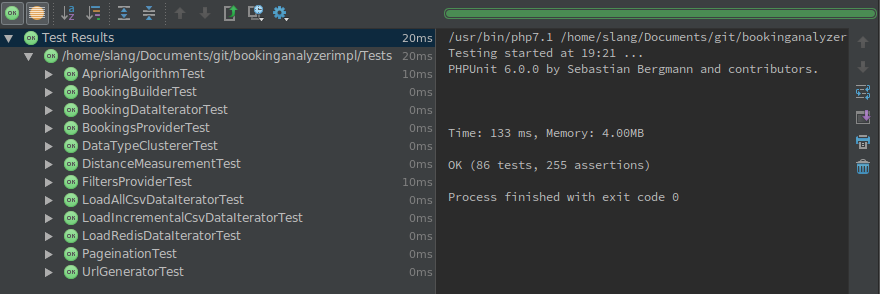
\includegraphics[width=1\textwidth]{images/unittests}
	\caption{Auswertungen der UnitTests}
	\label{fig:proofofconcept:unittests:1}
\end{figure}

Insgesammt wurden 86 Testfälle definiert, welche die Klassen in den Packages "`Business"' und "`Utilities"' abdecken. Die Models wurden nicht getestet da sie nur zur Datenhaltung verwendet werden und keine Logik enthalten. Leider konnten die Controller nicht mit UnitTests abgedeckt werden, da sie externe Abhängigkeiten zu den Services beinhalten. Würde ein Test ausgeführt werden, so hätte das zur folge dass ein Service, somit eine Analyse, gestartet würde.

Um den Dateizugriff der Iteratoren (siehe \cref{sec:proofofconcept:klassenstruktur:algorithmen} \nameref{sec:proofofconcept:klassenstruktur:algorithmen}) zu testen wurde die externe Bibliothek "`vfsStream"' verwendet. Dies erzeugt ein VFS (Virtual File Stream). Damit greift der Test nicht auf ein File auf dem Computer zu, sondern auf ein virtuelles Dateisystem.

\section{Installation}
In diesem Abschnitt wird die Installation des Proof of Concepts beschrieben. Beschrieben wird die Einrichtung für ein Linux auf Debian Basis. Es ist jedoch übertragbar auf alle Betriebssysteme.

Um das Programm zu installieren wird PHP 7 und Redis benötigt. Zusätzlich müssen noch alle externen Bibliotheken mit Composer geladen werden. Zuerst werden die Kommandozeilen-Befehle aufgeführt mit einer nachträglichen Erklärung. 

\begin{enumerate}
\item sudo apt-get apache2
\item sudo add-apt-repository ppa:ondrej/php
\item sudo apt-get update
\item sudo apt-get install php7.1-dev php-pear php7.1-mbstring php7.1-cgi
\end{enumerate}
Befehl 1. installiert einen Apache Webserver (siehe \url{https://httpd.apache.org/}). Die restlichen Kommandos werden benötigt um \gls{php} und all seine Abhängigkeiten zu installieren. 

Der Sourcecode des Programmes ist auf Github abgelegt (siehe \url{https://github.com/soultemptation/bookinganalyzerimpl}). Dieser muss für die Ausführung heruntergeladen werden. Dies kann entweder auf der Github Seite gemacht werden oder über die Kommandozeile. Für letzteres sollte zuerst dort hin navigiert werden, wo der Quellcode heruntergeladen werden soll. Dann kann folgender Befehl ausgeführt werden.
\begin{enumerate}[resume]
\item git clone git@github.com:soultemptation/bookinganalyzerimpl.git
\end{enumerate}

Danach können alle Abhängigkeiten des Programmes mittels Composer heruntergeladen werden. Dazu sollte die Kommandozeile im Ordner des Quellcodes stehen. Danach folgender Befehl ausführen.
\begin{enumerate}[resume]
\item php composer.phar update
\end{enumerate}

Als letztes muss Redis installiert und die Buchungsdaten in die Redis Datenbank importiert werden (siehe \cref{sec:proofofconcept:performance:datenzugriff} \nameref{sec:proofofconcept:performance:datenzugriff}).

\begin{enumerate}[resume]
\item sudo pecl install redis
\item sudo bash -c "echo extension=redis.so > /etc/php/7.X/apache2/redis.ini"
\item sudo bash -c "echo extension=redis.so > /etc/php/7.X/cli/redis.ini"
\item sudo /etc/init.d/apache2 restart
\item php Services/FillRedis/fillredis.php
\end{enumerate}

Befehl 7 installiert Redis als \gls{php} Erweiterung. Anschliessend wird mit dem Kommando 8 und 9 die Erweiterung in \gls{php} registriert. Schlussendlich wird der Apache Server neu gestartet und darauf hin der FillRedis Service gestartet.

Danach kann im Browser unter der Adresse "`http://localhost"' das Programm gestartet werden.

\section{Konfiguration}
\label{sec:proofofconcept:konfiguration}
Zur Konfigurierung der Algorithmen kann die "`Einstellungen anpassen"' Ansicht des Programmes aufgerufen werden. Es können jedoch noch mehr Konfigurationen vorgenommen werden, welche nicht für die Endbenutzer gedacht sind. Zum Beispiel was für Felder in der Datenbasis verwendet werden sollen, wie die diskretierung der Felder auf die ursprünglichen Werte zurückgerechnet werden kann, etc. 

Die Konfigurationen sind im File "`config.php"' hinterlegt (siehe \url{https://github.com/soultemptation/bookinganalyzerimpl/blob/master/config.php}). Die Struktur ist ein \gls{php} Array. Nachfolgend werden die Felder beschrieben.

\begin{itemize}
\item dataSource: Pfad zum \gls{csv} File welches alle Buchungen enthält.
\item pageSize: Wie viel Resultate in der "`Stammdaten einsehen"' Ansicht angezeigt werden.
\item paginationWindow: Wie viele Seiten unterhalb der Resultate in der "`Stammdaten einsehen"' Ansicht angezeigt werden.
\item booleanFields: Welche Felder in der Datenbasis werden als Binäre-Werte interpretiert.
\item integerFields: Welche Felder in der Datenbasis werden als Zahlen-Werte interpretiert.
\item floatFields: Welche Felder in der Datenbasis werden als Fliesskomma-Werte interpretiert.
\item stringFields: Welche Felder in der Datenbasis werden als Text-Werte interpretiert.
\item priceFields: Welche Felder in der Datenbasis werden als Preis-Werte interpretiert.
\item distanceFields: Welche Felder in der Datenbasis werden als Distanz-Werte interpretiert.
\item floatFieldsBoundaries: Alle Flieskomma-Werte sind das Resultat einer diskretierung. Um diese dem Benutzer angezeigt werden muss die Diskretierung zurückgerechnet werden. Dieses Feld definiert wie das Resultat der Diskretierung rückgängig gemacht werden kann.
\item atLeastFilterFields: Es gibt Felder welche einen "`Ab"'-Wert beinhalten. Zum Beispiel soll für den Filter "`Zimmer"' mit dem Wert "`3+"' alle Instanzen ausgewählt werden, welche 3 oder mehr Zimmer beinhalten. Dieses Feld definiert, für welche Felder solch eine "`Ab"'-Suche durchgeführt werden soll.
\item fieldNameMapping: Dieses Feld beinhaltet die Namen der Felder. Dem Benutzer wird somit anstelle des Feldes "`CUCNTRY"' der Name "`Customer Country"' angezeigt.
\item fileCacheDirectory: Beinhaltet den Pfad zu den Cache Dateien.
\item apriori: Beinhaltet alle Konfigurationen für den Apriori Algorithmus.
\item kprototype: Beinhaltet alle Konfigurationen für den k-prototype Algorithmus.
\item dbscan: Beinhaltet alle Konfigurationen für den DBSCAN Algorithmus.
\end{itemize}

Wenn in der Datenbasis ein neues Feld hinzugefügt wird, so kann es in der Konfiguration erweitert werden und es wird automatisch in den Algorithmen verwendet. Dazu muss es in einem der Felder "`booleanFields"', "`integerfields"', "`floatFields"', "`stringFields"', "`priceFields"' oder "`distancefields"' hinzugefügt werden. Ist ein diskretiertes Feld, so muss zusätzlich noch ein Eintrag im Feld "`floatFieldsBoundaries"' erstellt werden.


\section{Fazit}
\label{sec:proofofconcept:fazit}
Implementiert wurden eine Webanwendung mittels \gls{php}. Im \cref{app:pocansichten} wird die Programmoberfläche der Umsetzung gezeigt. Den grössten Einfluss auf die Entwicklung hatten die Anforderungen aus dem Konzept (siehe \cref{sec:proofofconcept:architektur:anforderungen} \nameref{sec:proofofconcept:architektur:anforderungen}) sowie die Laufzeit der Algorithmen. Da diese länger als 30 Sekunden dauern wurde die Berechnung in Hintergrundprozesse ausgelagert. Nichts desto trotz wurde eine Lösung erstellt, welche Modular aufgebaut ist (siehe \cref{sec:proofofconcept:packagestruktur} \nameref{sec:proofofconcept:packagestruktur}) und leicht durch weitere Attribute erweitert werden kann (siehe \cref{sec:proofofconcept:konfiguration} \nameref{sec:proofofconcept:konfiguration}). Um die Applikation um einen Algorithmus zu erweitern kann ein weiterer Service hinzugefügt werden (siehe \cref{sec:proofofconcept:architektur:services} \nameref{sec:proofofconcept:architektur:services}).

Erste Analysen welche mit dem Programm durchgeführt wurden zeigten auf, dass der Apriori-Algorithmus sehr hilfreich ist, je spezifischer die Anfrage gestellt wird. Bei einer Apriori Analyse der gesamte Datenbasis mit allen Attributen ist das Resultat nicht sonderlich aussagekräftig. 

\begin{figure}[H]
	\RawFloats
	\centering
	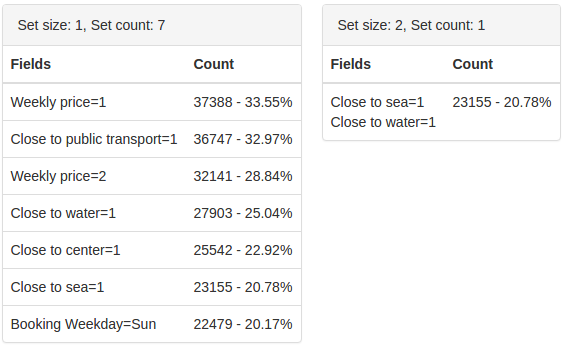
\includegraphics[width=1\textwidth]{images/result-of-everything}
	\caption{Resultat der Apriori Analyse mit allen Buchungen und sämtlichen Attributen}
	\label{fig:proofofconcept:fazit:1}
\end{figure}

Bessere Resultate erhält man, wenn die Datenbasis eingeschränkt wird. Zum Beispiel wenn man nur Kunden aus der Schweiz in der Analyse verwendet. Anschliessend kann man dasselbe für Kunden aus Frankreich machen und die beiden Resultate gegeneinander vergleichen. Auch hilfreich ist die Einschränkung der Attribute, welche in die Analyse einfliessen. Zuerst angedacht war in der Arbeit, dass die Algorithmen möglichst oft mit möglichst vielen Attributen arbeiten. Bei der Auswertung der Hypothesen (siehe \cref{sec:einleitung:ziel:hypothesen} \nameref{sec:einleitung:ziel:hypothesen}) hat sich jedoch gezeigt dass viele Fragestellungen nur wenige Attribute benötigen. Besonders oft wurden die Wochentage, Monate, Destinationen des Objektes und des Kunden sowie die Distanzen verwendet. Die Restlichen Attribute werden in Zukunft hoffentlich bei der Analyse durch Interhome verwendet. Ansonsten können diese leicht durch eine Konfigurationsänderung entfernt werden.

Die grösste Stärke des Apriori Algorithmus ist dessen Geschwindigkeit. Je höher der $minsup$ ist, desto schneller Arbeitet er. Bei ein Wert von 0.1 dauert eine Analyse im Durchschnitt 32 Sekunden über die gesamte Datenbasis mit allen Attributen. Das lädt ein verschiedene Kombinationen an Filtern auszuprobieren um ein brauchbares Resultat zu finden. Die Clustering Algorithmen hingegen sind sehr langsam. Wenn die Analyse auf 1'500 Instanzen eingeschränkt wird dauert ein Durchlauf bereits über 20 Minuten. Das Negative daran ist die exponentielle Laufzeit. 3'000 Instanzen brauchen demnach nicht 40 Minuten, sondern bereits Stunden. Nicht gerade hilfreich ist dabei die Tatsache, dass mehrere verschiedene Parameter die Analyse massiv beeinträchtigen (siehe \cref{sec:recherche:algorithmen:k-prototypes} \nameref{sec:recherche:algorithmen:k-prototypes} und \cref{sec:recherche:algorithmen:dbscan} \nameref{sec:recherche:algorithmen:dbscan}). Im \cref{sec:konzept:parameterauswahl} \nameref{sec:konzept:parameterauswahl} wurde zum Beispiel die Elbow-Methode zur Erhebung eines geeigneten $k$ Wertes vorgenommen. Jedoch ist dies bei der Laufzeit der Algorithmen nicht möglich weshalb sie nicht umgesetzt wurde. Die Parameter $\epsilon$, $minpts$ und $\gamma$ sollen explorativ ermittelt werden. Jedoch ist dies bei diesen Laufzeiten nicht praktikabel. 

Nichts desto trotz wurden Durchläufe der Clustering Algorithmen ausgeführt. Die Resultate waren jedoch nicht besonders aufschlussreich. Der k-prototype findet per Definition immer $k$ Cluster. Erwartet wurde, dass einige Attribute in einer Gruppe sehr oft vertreten sind, und in einer anderen möglichst selten. Jedoch zeigten die Resultate die selben Attribute oft in beiden Clustern mit ähnlicher Häufigkeit, womit keine klaren Schlüsse gezogen werden konnten. Der DBSCAN findet auf den Daten von Interhome entweder nur einen Cluster, oder einen grösseren Cluster und ganz viele Noise Punkte. Entweder benötigen die Clustering Algorithmen noch weitere Feineinstellungen der Parameter, oder es sind schlichtweg keine eindeutigen Cluster in den Daten zu finden. Die Resultate lassen aber letzteres Vermuten. Denn dieses Verhalten wäre erklärbar, wenn viele Instanzen zueinander ähnlich sind und es nur wenige Ausreisser gibt. In \cref{fig:proofofconcept:fazit:2} wird die vermutete Verhalten der Buchungen in der Datenbasis Beispielhaft auf einem Koordinatensytem aufgezeigt. Grüne Punkte gehören zu einem Cluster und sind alle sehr ähnlich zu einander und irgendwo in der Mitte angesiedelt. Ausserhalb der Hauptgruppe gibt es wenige Ausreisser, welche jedoch untereinander keinen Cluster bilden können. Dann würde der k-prototype $k$ Clusters finden, diese jedoch nicht klar unterscheiden könne. Der DBSCAN findet bei solch einer Verteilung nur eine Gruppe und einige Noise Punkte.

\begin{figure}[H]
	\RawFloats
	\centering
	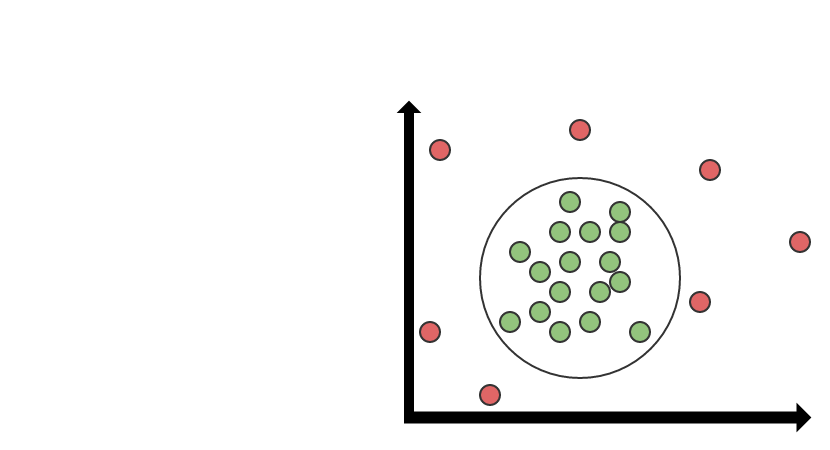
\includegraphics[width=0.6\textwidth]{images/expected-data-distribution}
	\caption{Vermutete Verteilung der Buchungen in der Datenbasis}
	\label{fig:proofofconcept:fazit:2}
\end{figure}

